\documentclass[12pt,a4paper]{article}
\usepackage{lmodern}
\usepackage{graphicx}
\usepackage{fancyhdr}
\usepackage[T1]{fontenc}
\usepackage[croatian]{babel}
\usepackage[left=3.5cm, top=3.5cm, right=3cm, bottom=3cm]{geometry}
\linespread{1.5}
\usepackage{amsfonts}
\usepackage{amsmath}
\usepackage{hyperref}
\hypersetup{hidelinks}
\usepackage{pgfplots}
\pgfplotsset{compat=1.18}
\usepgfplotslibrary{colormaps}
\usepackage{bm}
\usepackage{amsthm}
\usepackage[bottom]{footmisc}
\interfootnotelinepenalty=10000

\newtheorem{tm}{Teorem}[section]
\newtheorem{pr}[tm]{Primjer}
\newtheorem{lema}[tm]{Lema}
\newtheorem{deff}[tm]{Definicija}
\newtheorem{napomena}[tm]{Napomena}

\usepackage{caption}
\captionsetup[figure]{justification=centering}
\usepackage{tikz}
\usepackage{tikz-3dplot}
\usepackage{float}
\usepackage{amsmath,amssymb}
\usetikzlibrary{arrows.meta,3d}
\usetikzlibrary{
    shapes.geometric,
    shadings,
    intersections,
    calc,
    decorations.markings,
    patterns
}
\usepackage{tocloft}

\setlength{\cftbeforesecskip}{10pt}
\setlength{\cftbeforesubsecskip}{3pt}
\setlength{\cftbeforesubsubsecskip}{3pt}
\setlength{\parindent}{0pt}


\makeatletter

\renewenvironment{proof}[1][\proofname]{\par
  \pushQED{\qed}%
  \normalfont
  \topsep6\p@\@plus6\p@\relax
  \trivlist
  \item[\hskip\labelsep
  \bfseries #1\@addpunct{.}]\ignorespaces
}{%
  \popQED\endtrivlist\@endpefalse
}


\tikzset{
    volumen/.style={
        fill=blue!10,
        draw=blue!40!black!60,
        dashed,
        opacity=0.7
    },
    sjena_volumena/.style={
        shading=ball,
        ball color=blue!10,
        opacity=0.5
    },
    sjena_dif/.style={
        shading=ball,
        ball color=gray!30,
        opacity=0.8
    },
    poljestrelica/.style={
        ->,
        >={Latex[length=1.4mm,width=0.9mm]},
        line width=0.30pt,
        black!65
    },
    poljestrelicaMala/.style={
        ->,
        >={Latex[length=1.4mm,width=0.9mm]},
        line width=0.30pt,
        black!65
    },
    silnicaplava/.style={
        ->,
        >={Latex[length=1.3mm,width=0.95mm]},
        line width=0.28pt,
        blue!70!black,
        line cap=round,
        line join=round
    },
    silnicaplavaSlaba/.style={
        ->,
        >={Latex[length=1.2mm,width=0.85mm]},
        line width=0.24pt,
        blue!55!black,
        line cap=round,
        line join=round
    },
    silnicacrvena/.style={
        ->,
        >={Latex[length=1.3mm,width=0.95mm]},
        line width=0.28pt,
        red!70!black,
        line cap=round,
        line join=round
    },
    silnicacrvenaSlaba/.style={
        ->,
        >={Latex[length=1.2mm,width=0.85mm]},
        line width=0.24pt,
        red!55!black,
        line cap=round,
        line join=round
    }
}

\pgfplotsset{
    os3d/.style={
        axis lines=center,
        axis line style={
            ->,
            >={Latex[length=2mm,width=1.5mm]},
            line width=0.70pt,
            black!65
        },
        xmin=-2.5,
        xmax=2.5,
        ymin=-2.5,
        ymax=2.5,
        zmin=-2.5,
        zmax=2.5,
        ticks=none,
        grid=none,
        clip=false
    }
}

\makeatother

\newcommand{\StrelicePoljaF}{
    \foreach \x in {-1.5,-0.5,0.5,1.5}{
        \foreach \y in {-1.5,-0.5,0.5,1.5}{
            \foreach \z in {-1.5,-0.5,0.5,1.5}{

                \pgfmathsetmacro{\nazivnik}
                    {(1+\x*\x+\y*\y+\z*\z)^2}

                \pgfmathsetmacro{\Fx}
                    {2*\x*(\z+1)/\nazivnik}

                \pgfmathsetmacro{\Fy}
                    {2*\y*(\z+1)/\nazivnik}

                \pgfmathsetmacro{\Fz}
                    {2*(\z*\z+\z+1)/\nazivnik}

                \pgfmathsetmacro{\Fnorma}
                    {sqrt(\Fx*\Fx+\Fy*\Fy+\Fz*\Fz)}

                \pgfmathsetmacro{\duljina}
                    {0.25 + 0.28*\Fnorma/(0.4+\Fnorma)}

                \pgfmathsetmacro{\Xkraj}
                    {\x+\duljina*\Fx/\Fnorma}

                \pgfmathsetmacro{\Ykraj}
                    {\y+\duljina*\Fy/\Fnorma}

                \pgfmathsetmacro{\Zkraj}
                    {\z+\duljina*\Fz/\Fnorma}

                \edef\temp{
                    \noexpand\draw[poljestrelica]
                    (axis cs:\x,\y,\z) --
                    (axis cs:\Xkraj,\Ykraj,\Zkraj);
                }

                \temp
            }
        }
    }
}

\newcommand{\SilnicePoljaF}{

    \draw[silnicaplava]
        (axis cs:-1.45,0,-1.75)
        .. controls
        (axis cs:-0.34,0,-0.85)
        and
        (axis cs:-0.38,0,0.82)
        ..
        (axis cs:-1.28,0,1.82);

    \draw[silnicaplava]
        (axis cs:1.45,0,-1.75)
        .. controls
        (axis cs:0.34,0,-0.85)
        and
        (axis cs:0.38,0,0.82)
        ..
        (axis cs:1.28,0,1.82);

    \draw[silnicaplava]
        (axis cs:0,-1.45,-1.75)
        .. controls
        (axis cs:0,-0.34,-0.85)
        and
        (axis cs:0,-0.38,0.82)
        ..
        (axis cs:0,-1.28,1.82);

    \draw[silnicaplava]
        (axis cs:0,1.45,-1.75)
        .. controls
        (axis cs:0,0.34,-0.85)
        and
        (axis cs:0,0.38,0.82)
        ..
        (axis cs:0,1.28,1.82);

    \draw[silnicaplavaSlaba]
        (axis cs:-1.02,-1.02,-1.75)
        .. controls
        (axis cs:-0.24,-0.24,-0.85)
        and
        (axis cs:-0.28,-0.28,0.82)
        ..
        (axis cs:-0.92,-0.92,1.82);

    \draw[silnicaplavaSlaba]
        (axis cs:1.02,1.02,-1.75)
        .. controls
        (axis cs:0.24,0.24,-0.85)
        and
        (axis cs:0.28,0.28,0.82)
        ..
        (axis cs:0.92,0.92,1.82);
}

\newcommand{\StreliceGradU}{
    \foreach \x in {-1.5,-0.5,0.5,1.5}{
        \foreach \y in {-1.5,-0.5,0.5,1.5}{
            \foreach \z in {-1.5,-0.5,0.5,1.5}{

                \pgfmathsetmacro{\nazivnik}
                    {(1+\x*\x+\y*\y+\z*\z)^2}

                \pgfmathsetmacro{\Fx}
                    {2*\x/\nazivnik}

                \pgfmathsetmacro{\Fy}
                    {2*\y/\nazivnik}

                \pgfmathsetmacro{\Fz}
                    {2*\z/\nazivnik}

                \pgfmathsetmacro{\Fnorma}
                    {sqrt(\Fx*\Fx+\Fy*\Fy+\Fz*\Fz)}

                \pgfmathsetmacro{\duljina}
                    {0.22 + 0.28*\Fnorma/(0.35+\Fnorma)}

                \pgfmathsetmacro{\Xkraj}
                    {\x+\duljina*\Fx/\Fnorma}

                \pgfmathsetmacro{\Ykraj}
                    {\y+\duljina*\Fy/\Fnorma}

                \pgfmathsetmacro{\Zkraj}
                    {\z+\duljina*\Fz/\Fnorma}

                \edef\temp{
                    \noexpand\draw[poljestrelicaMala]
                    (axis cs:\x,\y,\z) --
                    (axis cs:\Xkraj,\Ykraj,\Zkraj);
                }

                \temp
            }
        }
    }
}

\newcommand{\SilniceGradU}{

    \draw[silnicacrvena]
        (axis cs:0.08,0,0) --
        (axis cs:1.70,0,0);

    \draw[silnicacrvena]
        (axis cs:-0.08,0,0) --
        (axis cs:-1.70,0,0);

    \draw[silnicacrvena]
        (axis cs:0,0.08,0) --
        (axis cs:0,1.70,0);

    \draw[silnicacrvena]
        (axis cs:0,-0.08,0) --
        (axis cs:0,-1.70,0);

    \draw[silnicacrvena]
        (axis cs:0,0,0.08) --
        (axis cs:0,0,1.70);

    \draw[silnicacrvena]
        (axis cs:0,0,-0.08) --
        (axis cs:0,0,-1.70);

    \draw[silnicacrvenaSlaba]
        (axis cs:0.08,0.08,0) --
        (axis cs:1.35,1.35,0);

    \draw[silnicacrvenaSlaba]
        (axis cs:-0.08,-0.08,0) --
        (axis cs:-1.35,-1.35,0);

    \draw[silnicacrvenaSlaba]
        (axis cs:0.08,-0.08,0) --
        (axis cs:1.35,-1.35,0);

    \draw[silnicacrvenaSlaba]
        (axis cs:-0.08,0.08,0) --
        (axis cs:-1.35,1.35,0);

    \draw[silnicacrvenaSlaba]
        (axis cs:0.08,0,0.08) --
        (axis cs:1.35,0,1.35);

    \draw[silnicacrvenaSlaba]
        (axis cs:-0.08,0,-0.08) --
        (axis cs:-1.35,0,-1.35);

    \draw[silnicacrvenaSlaba]
        (axis cs:0.08,0,-0.08) --
        (axis cs:1.35,0,-1.35);

    \draw[silnicacrvenaSlaba]
        (axis cs:-0.08,0,0.08) --
        (axis cs:-1.35,0,1.35);

    \draw[silnicacrvenaSlaba]
        (axis cs:0,0.08,0.08) --
        (axis cs:0,1.35,1.35);

    \draw[silnicacrvenaSlaba]
        (axis cs:0,-0.08,-0.08) --
        (axis cs:0,-1.35,-1.35);

    \draw[silnicacrvenaSlaba]
        (axis cs:0,0.08,-0.08) --
        (axis cs:0,1.35,-1.35);

    \draw[silnicacrvenaSlaba]
        (axis cs:0,-0.08,0.08) --
        (axis cs:0,-1.35,1.35);

    \draw[silnicacrvenaSlaba]
        (axis cs:0.07,0.07,0.07) --
        (axis cs:1.10,1.10,1.10);

    \draw[silnicacrvenaSlaba]
        (axis cs:-0.07,-0.07,-0.07) --
        (axis cs:-1.10,-1.10,-1.10);

    \draw[silnicacrvenaSlaba]
        (axis cs:0.07,-0.07,0.07) --
        (axis cs:1.10,-1.10,1.10);

    \draw[silnicacrvenaSlaba]
        (axis cs:-0.07,0.07,-0.07) --
        (axis cs:-1.10,1.10,-1.10);

    \draw[silnicacrvenaSlaba]
        (axis cs:0.07,0.07,-0.07) --
        (axis cs:1.10,1.10,-1.10);

    \draw[silnicacrvenaSlaba]
        (axis cs:-0.07,-0.07,0.07) --
        (axis cs:-1.10,-1.10,1.10);

    \draw[silnicacrvenaSlaba]
        (axis cs:-0.07,0.07,0.07) --
        (axis cs:-1.10,1.10,1.10);

    \draw[silnicacrvenaSlaba]
        (axis cs:0.07,-0.07,-0.07) --
        (axis cs:1.10,-1.10,-1.10);
}

\newcommand{\StreliceCurlW}{
    \foreach \x in {-1.5,-0.5,0.5,1.5}{
        \foreach \y in {-1.5,-0.5,0.5,1.5}{
            \foreach \z in {-1.5,-0.5,0.5,1.5}{

                \pgfmathsetmacro{\nazivnik}
                    {(1+\x*\x+\y*\y+\z*\z)^2}

                \pgfmathsetmacro{\Fx}
                    {2*\x*\z/\nazivnik}

                \pgfmathsetmacro{\Fy}
                    {2*\y*\z/\nazivnik}

                \pgfmathsetmacro{\Fz}
                    {2*(\z*\z+1)/\nazivnik}

                \pgfmathsetmacro{\Fnorma}
                    {sqrt(\Fx*\Fx+\Fy*\Fy+\Fz*\Fz)}

                \pgfmathsetmacro{\duljina}
                    {0.22 + 0.28*\Fnorma/(0.35+\Fnorma)}

                \pgfmathsetmacro{\Xkraj}
                    {\x+\duljina*\Fx/\Fnorma}

                \pgfmathsetmacro{\Ykraj}
                    {\y+\duljina*\Fy/\Fnorma}

                \pgfmathsetmacro{\Zkraj}
                    {\z+\duljina*\Fz/\Fnorma}

                \edef\temp{
                    \noexpand\draw[poljestrelicaMala]
                    (axis cs:\x,\y,\z) --
                    (axis cs:\Xkraj,\Ykraj,\Zkraj);
                }

                \temp
            }
        }
    }
}

\newcommand{\SilniceCurlW}{

    \draw[silnicaplava]
        (axis cs:0,0,-1.85) --
        (axis cs:0,0,1.85);

    \draw[silnicaplava]
        (axis cs:-0.85,0,-1.75)
        .. controls
        (axis cs:-0.22,0,-0.75)
        and
        (axis cs:-0.24,0,0.70)
        ..
        (axis cs:-0.85,0,1.75);

    \draw[silnicaplava]
        (axis cs:0.85,0,-1.75)
        .. controls
        (axis cs:0.22,0,-0.75)
        and
        (axis cs:0.24,0,0.70)
        ..
        (axis cs:0.85,0,1.75);

    \draw[silnicaplavaSlaba]
        (axis cs:-1.55,0,-1.80)
        .. controls
        (axis cs:-0.42,0,-0.75)
        and
        (axis cs:-0.45,0,0.70)
        ..
        (axis cs:-1.45,0,1.80);

    \draw[silnicaplavaSlaba]
        (axis cs:1.55,0,-1.80)
        .. controls
        (axis cs:0.42,0,-0.75)
        and
        (axis cs:0.45,0,0.70)
        ..
        (axis cs:1.45,0,1.80);
        
    \draw[silnicaplava]
        (axis cs:0,-0.85,-1.75)
        .. controls
        (axis cs:0,-0.22,-0.75)
        and
        (axis cs:0,-0.24,0.70)
        ..
        (axis cs:0,-0.85,1.75);

    \draw[silnicaplava]
        (axis cs:0,0.85,-1.75)
        .. controls
        (axis cs:0,0.22,-0.75)
        and
        (axis cs:0,0.24,0.70)
        ..
        (axis cs:0,0.85,1.75);

    \draw[silnicaplavaSlaba]
        (axis cs:0,-1.55,-1.80)
        .. controls
        (axis cs:0,-0.42,-0.75)
        and
        (axis cs:0,-0.45,0.70)
        ..
        (axis cs:0,-1.45,1.80);

    \draw[silnicaplavaSlaba]
        (axis cs:0,1.55,-1.80)
        .. controls
        (axis cs:0,0.42,-0.75)
        and
        (axis cs:0,0.45,0.70)
        ..
        (axis cs:0,1.45,1.80);

    \draw[silnicaplavaSlaba]
        (axis cs:-1.05,-1.05,-1.70)
        .. controls
        (axis cs:-0.27,-0.27,-0.70)
        and
        (axis cs:-0.30,-0.30,0.70)
        ..
        (axis cs:-0.98,-0.98,1.70);

    \draw[silnicaplavaSlaba]
        (axis cs:1.05,1.05,-1.70)
        .. controls
        (axis cs:0.27,0.27,-0.70)
        and
        (axis cs:0.30,0.30,0.70)
        ..
        (axis cs:0.98,0.98,1.70);

    \draw[silnicaplavaSlaba]
        (axis cs:1.05,-1.05,-1.70)
        .. controls
        (axis cs:0.27,-0.27,-0.70)
        and
        (axis cs:0.30,-0.30,0.70)
        ..
        (axis cs:0.98,-0.98,1.70);

    \draw[silnicaplavaSlaba]
        (axis cs:-1.05,1.05,-1.70)
        .. controls
        (axis cs:-0.27,0.27,-0.70)
        and
        (axis cs:-0.30,0.30,0.70)
        ..
        (axis cs:-0.98,0.98,1.70);
}
\begin{document}
\hypersetup{pageanchor=false}
\pagenumbering{gobble}

\begin{center}
    \textmd{\bfseries \large SVEUČILIŠTE U MOSTARU\\ [0.25cm]FAKULTET PRIRODOSLOVNO-MATEMATIČKIH I ODGOJNIH ZNANOSTI}\\ [0.25cm]
    \textsc{\bfseries \large MATEMATIKA I INFORMATIKA} \\[3.5cm]
    {\large \textbf{VEDRAN BOŠNJAK}}\\[1.5cm]
    {\large \textbf{HELMHOLTZOVA DEKOMPOZICIJA U $\mathbb{R}^3$ ZA GLATKA I BRZO OPADAJUĆA}}\\
    {\textbf{\large VEKTORSKA POLJA}}\\[1.5cm]
    {\large \textbf{ZAVRŠNI RAD}}

    \vspace*{\fill}
    {\large \textbf{Mostar, 2026.}}
\end{center}

\clearpage
\begin{center}
    \textmd{\bfseries \large SVEUČILIŠTE U MOSTARU\\ [0.25cm]FAKULTET PRIRODOSLOVNO-MATEMATIČKIH I ODGOJNIH ZNANOSTI}\\ [0.25cm]
    \textsc{\bfseries \large MATEMATIKA I INFORMATIKA} \\[3.5cm]
    {\large \textbf{HELMHOLTZOVA DEKOMPOZICIJA U $\mathbb{R}^3$ ZA GLATKA I BRZO OPADAJUĆA}}\\
    {\textbf{\large VEKTORSKA POLJA}}\\[1.5cm]
    {\large \textbf{ZAVRŠNI RAD}}\\[1.5cm]
    {\large \textbf{doc. dr. sc. Ivančica Mirošević}}

    {\large \textbf{Vedran Bošnjak}}

    \vspace*{\fill}
    {\large \textbf{Mostar, 2026.}}
\end{center}

\clearpage
\begin{center}
    \normalsize{\textbf{PODACI O ZAVRŠNOM RADU}}
\end{center}
\normalsize{\textbf{I. AUTOR}}
\vspace{0.8cm}
\\Ime i prezime: Vedran Bošnjak
\\Datum i mjesto rođenja: 11.07.2004., Mostar
\\Studentska grupa: Matematika i Informatika
\vspace{1cm}
\\ \normalsize{\textbf{II. ZAVRŠNI RAD}}
\vspace{0.8cm}
\\Tema: \textbf{Helmholtzova dekompozicija u $\mathbb{R}^3$ za glatka i brzo opadajuća vektorska polja}
\\Broj stranica: 32
\\Datum predaje završnog rada:
\\Datum obrane završnog rada:
\\Mentorica: dr. sc. Ivančica Mirošević, doc.
\vspace{1cm}
\\ \normalsize{\textbf{Sastav povjerenstva koje je ocijenilo rad:}}
\vspace{0.8cm}
\\Mentorica: dr. sc. Ivančica Mirošević, doc.
\vspace{0.5cm}
\\Potpis mentorice: \makebox[5cm]{\hrulefill}
\vspace{1cm}
\\Ocjena završnog rada i ocjena obrane: \makebox[5cm]{\hrulefill}

\clearpage
\tableofcontents
\clearpage

\section*{Sažetak}

U ovom radu razmatra se Helmholtzova dekompozicija glatkih i brzo
opadajućih vektorskih polja u prostoru $\mathbb{R}^3$. Najprije se uvode
osnovni pojmovi vektorske analize potrebni za formulaciju i dokaz glavnog
rezultata: skalarna i vektorska polja, gradijent, divergencija, rotacija,
Laplaceov diferencijalni operator, harmonijske funkcije te krivuljni i plošni integrali.
Posebno se navode teorem o divergenciji, Greenov drugi identitet i Stokesov teorem, a zatim se uvodi
Newtonov potencijal i dokazuje njegova povezanost s Poissonovom jednadžbom.
Na toj se osnovi dokazuje Helmholtzov teorem, kojim se vektorsko polje
rastavlja na bezvrtložni i solenoidalni dio, te se dokazuje jedinstvenost
polja određenog divergencijom i rotacijom uz odgovarajuće uvjete u
beskonačnosti. Dekompozicija se zatim prikazuje na dvama primjerima, od kojih
jedan sadrži samo solenoidalni dio, dok drugi sadrži i bezvrtložni i
solenoidalni dio. Na kraju se razmatraju primjene u elektrostatici,
magnetostatici, gravitacijskom polju i dinamici fluida.

\section*{Ključne riječi}

Helmholtzova dekompozicija, vektorsko polje, divergencija, rotacija,
skalarni potencijal, vektorski potencijal

\newpage
\hypersetup{pageanchor=true}
\pagenumbering{arabic}
\setcounter{page}{1}

\section{Uvod}

Vektorska polja imaju važnu ulogu u matematici i fizici jer se njima mogu
opisivati električna i magnetska polja, gravitacijsko polje te gibanje
fluida. Pri njihovu proučavanju posebno je važno odrediti kako su lokalna
svojstva polja, ponajprije divergencija i rotacija, povezana s njegovom
globalnom strukturom.

Tu vezu opisuje Helmholtzov teorem. Uz odgovarajuće uvjete
glatkoće i opadanja u beskonačnosti, vektorsko se polje može rastaviti na
bezvrtložni dio određen skalarnim potencijalom i solenoidalni dio određen
vektorskim potencijalom. 

Počeci tih ideja povezani su s radom Hermanna von Helmholtza\footnote{Hermann Ludwig
Ferdinand von Helmholtz (1821.--1894.),
njemački fizičar i liječnik.}, koji je 1858. u radu
\textit{Über Integrale der hydrodynamischen Gleichungen, welche den
Wirbelbewegungen entsprechen} proučavao vrtložna gibanja
fluida i time postavio važne temelje matematičke teorije vrtložnosti.

Cilj je ovog rada proučiti Helmholtzovu dekompoziciju glatkih i brzo opadajućih vektorskih polja u $\mathbb{R}^3$, dokazati njezino postojanje te pokazati da divergencija i rotacija, uz odgovarajući uvjet u beskonačnosti, jednoznačno određuju vektorsko polje.
Posebna se pozornost posvećuje ulozi brzog opadanja u beskonačnosti te
određivanju potencijala kojima se polje može rekonstruirati iz njegove
divergencije i rotacije.\newpage
\section{Temeljni pojmovi i teoremi vektorske analize}

Za formulaciju i dokaz Helmholtzova teorema potrebni su određeni pojmovi i rezultati vektorske analize. U ovom poglavlju uvodimo skalarna i vektorska polja, gradijent, divergenciju i rotaciju, Laplaceov diferencijalni operator, harmonijske funkcije, Newtonov potencijal te integralne teoreme koji će se koristiti u nastavku rada.


\subsection{Skalarna i vektorska polja}

\begin{deff}
Neka je $\Omega\subseteq\mathbb{R}^3$. Svaku funkciju
$$
f:\Omega\to\mathbb{R}
$$
nazivamo \textbf{\textit{skalarnim poljem}} na skupu $\Omega$.
\end{deff}

Skalarno polje svakoj točki prostora pridružuje jedan realan
broj.

\begin{deff}
Neka je $\Omega\subseteq\mathbb{R}^3$. Svaku funkciju
$$
\overrightarrow{F}:\Omega\to\mathbb{R}^3
$$
nazivamo \textbf{\textit{vektorskim poljem}} na skupu $\Omega$. Vektorsko polje
zapisujemo u obliku $$
\overrightarrow{F}=(F_x,F_y,F_z),
$$ odnosno
$$
\overrightarrow{F}
=
F_x\overrightarrow{i}
+
F_y\overrightarrow{j}
+
F_z\overrightarrow{k},
$$
gdje su $F_x,F_y,F_z:\Omega \to \mathbb{R}$ njegove skalarne komponente, a
$\overrightarrow{i},\overrightarrow{j},\overrightarrow{k}$ ortonormirani vektori baze vektorskog prostora $\mathbb{R}^3$.\end{deff}

Točku $T=(x,y,z)\in\mathbb{R}^3$ ćemo često zapisivati s pomoću njezina
radijvektora
$$
\overrightarrow{r}
=
x\overrightarrow{i}
+
y\overrightarrow{j}
+
z\overrightarrow{k},\ r=\|\overrightarrow{r}\|.
$$
Za skalarno polje $f$ tada možemo pisati
\[
f(x,y,z)=f(\overrightarrow{r})
\]
i analogno za vektorsko polje $\overrightarrow{F}$ možemo pisati
\[
\overrightarrow{F}(x,y,z)=\overrightarrow{F}(\overrightarrow{r}).
\]
\begin{deff}
Neka je $\Omega\subseteq\mathbb{R}^3$ otvoren skup i neka su
$T=(x,y,z)$ i
$T_0=(x_0,y_0,z_0)\in\Omega$.
Za skalarno polje $f:\Omega\to\mathbb{R}$ kažemo da je
\textbf{diferencijabilno} u točki $T_0$ ako se njegov prirast
$$
\Delta f
=
f(T)-f(T_0)
=
f(T_0+\Delta T)-f(T_0),
$$
gdje je
$$
\Delta T
=
(\Delta x,\Delta y,\Delta z),
$$
može zapisati u obliku
$$
\Delta f
=
\frac{\partial f}{\partial x}(T_0)\Delta x
+\frac{\partial f}{\partial y}(T_0)\Delta y+
\frac{\partial f}{\partial z}(T_0)\Delta z
+o(\|\Delta T\|),
$$
pri čemu
$$
\lim\limits_{\Delta T\to\overrightarrow{0}}
\frac{o(\|\Delta T\|)}{\|\Delta T\|}
=
0.
$$\\
Kažemo da je skalarno polje $f$ \textbf{diferencijabilno} na $\Omega$ ako je
diferencijabilno u svakoj točki $T_0\in\Omega$. Za vektorsko polje
$\overrightarrow{F}=(F_x,F_y,F_z):\Omega\to\mathbb{R}^3$
kažemo da je \textbf{diferencijabilno} na $\Omega$ ako su njegove
skalarne komponente $F_x,F_y,F_z$ diferencijabilne na $\Omega$.
\end{deff}
\begin{deff}
Neka je $\Omega\subseteq\mathbb{R}^3$ otvoren skup i neka je
$k\in\mathbb{N}$. Za skalarno polje
$f:\Omega\to\mathbb{R}$
kažemo da je \textbf{klase $C^k$} ako sve njegove parcijalne derivacije do
uključivo reda $k$ postoje i neprekidne su na $\Omega$. Za vektorsko polje
$\overrightarrow{F}=(F_x,F_y,F_z):\Omega\to\mathbb{R}^3$
kažemo da je \textbf{klase $C^k$} ako su njegove skalarne komponente
$F_x,F_y,F_z$ klase $C^k$ na $\Omega$.
\end{deff}
Postojanje i neprekidnost parcijalnih derivacija povlače diferencijabilnost,
pa je skalarno polje klase $C^k$ ujedno i $k$ puta diferencijabilno na
otvorenom skupu $\Omega$.

\begin{deff}
     Neka je \(f:\mathbb{R}^3\to\mathbb{R}\) funkcija klase \(C^2\).  Kažemo da je \(f\) \textbf{brzo opadajuća} ako postoje konstante \(C>0\) i \(\alpha>0\) takve da vrijedi\\
	$$ |f(\overrightarrow{r})|,\quad \left|\frac{\partial f}{\partial x_i}(\overrightarrow{r})\right|,\quad \left|\frac{\partial^2f}{\partial x_i\partial x_j}(\overrightarrow{r})\right| \le \frac{C}{(1+\|\overrightarrow{r}\|)^{2+\alpha}} $$\\
	za sve \(i,j\in\{1,2,3\}\). Za vektorsko polje
\(\ \overrightarrow{F}=(F_x,F_y,F_z):\mathbb{R}^3\to\mathbb{R}^3\) kažemo da je \textbf{brzo opadajuće} ako je svaka njegova komponenta brzo opadajuća.
	\end{deff}

    
\begin{napomena}
U literaturi se pojam brzo opadajuće funkcije često koristi u smislu
Schwartzovih funkcija, odnosno funkcija klase $C^\infty$ za koje funkcija
i sve njezine parcijalne derivacije opadaju brže od svake potencije
$\|\overrightarrow{r}\|^{-1}$ kada
$\|\overrightarrow{r}\|\to\infty$. Takav je uvjet za potrebe ovog rada nepotrebno jak. Stoga se u nastavku
izraz brzo opadajuća funkcija koristi isključivo u smislu prethodne
definicije.
\end{napomena}

\subsection{Gradijent, divergencija i rotacija}

\begin{deff}
Neka je $f:\Omega\to\mathbb{R}$, $\Omega \subseteq \mathbb{R}^3$ otvoren, diferencijabilno skalarno polje.
\textbf{\textit{Gradijentom}} skalarnog polja $f$ nazivamo vektorsko polje
$\operatorname{grad}f:\Omega\to\mathbb{R}^3$ definirano s
$$
\operatorname{grad}f(x,y,z)
=
\frac{\partial f(x,y,z)}{\partial x}\overrightarrow{i}
+
\frac{\partial f(x,y,z)}{\partial y}\overrightarrow{j}
+
\frac{\partial f(x,y,z)}{\partial z}\overrightarrow{k}.
$$
\end{deff}

\begin{figure}[H]
\centering
\colorlet{normcol}{blue!70!black}
\colorlet{sidecol}{violet!55!blue}
\colorlet{gradcol}{orange!85!red}
\def\thv{68}\def\phv{125}     
\tdplotsetmaincoords{\thv}{\phv}
\pgfmathsetmacro{\ea}{2.3} 
\pgfmathsetmacro{\eb}{1.6} 
\pgfmathsetmacro{\ec}{1.1} 
\pgfmathsetmacro{\k}{0.6} 
\begin{minipage}[t]{0.52\textwidth}
\centering
\begin{tikzpicture}[tdplot_main_coords, scale=1.25, line cap=round, line join=round]
  \pgfmathsetmacro{\vx}{sin(\thv)*sin(\phv)}
  \pgfmathsetmacro{\vy}{-sin(\thv)*cos(\phv)}
  \pgfmathsetmacro{\vz}{cos(\thv)}

  \foreach \ax/\ay/\az/\len in {1/0/0/3.3, 0/1/0/2.8, 0/0/1/2.6} {%
    \draw[-{Stealth[length=2.2mm,width=1.8mm]}, gray!55, line width=0.6pt]
      ({-\len*\ax},{-\len*\ay},{-\len*\az}) -- ({\len*\ax},{\len*\ay},{\len*\az});
  }

  \foreach \c/\shbase in {-0.45/38, 0/55, 0.45/74} {%
    \foreach \j in {0,...,11} {%
      \foreach \i in {0,...,15} {%
        \pgfmathsetmacro{\xa}{-\ea+2*\ea*\i/16}
        \pgfmathsetmacro{\xb}{-\ea+2*\ea*(\i+1)/16}
        \pgfmathsetmacro{\ya}{-\eb+2*\eb*\j/12}
        \pgfmathsetmacro{\yb}{-\eb+2*\eb*(\j+1)/12}
        \pgfmathsetmacro{\xm}{(\xa+\xb)/2}
        \pgfmathsetmacro{\ym}{(\ya+\yb)/2}
        \pgfmathsetmacro{\za}{\c+\ec*(\xa*\xa/(\ea*\ea)-\ya*\ya/(\eb*\eb))}
        \pgfmathsetmacro{\zb}{\c+\ec*(\xb*\xb/(\ea*\ea)-\ya*\ya/(\eb*\eb))}
        \pgfmathsetmacro{\zzc}{\c+\ec*(\xb*\xb/(\ea*\ea)-\yb*\yb/(\eb*\eb))}
        \pgfmathsetmacro{\zd}{\c+\ec*(\xa*\xa/(\ea*\ea)-\yb*\yb/(\eb*\eb))}
        \pgfmathsetmacro{\dzdx}{2*\ec*\xm/(\ea*\ea)}
        \pgfmathsetmacro{\dzdy}{-2*\ec*\ym/(\eb*\eb)}
        \pgfmathsetmacro{\nn}{sqrt(\dzdx*\dzdx+\dzdy*\dzdy+1)}
        \pgfmathsetmacro{\Nxc}{-\dzdx/\nn}
        \pgfmathsetmacro{\Nyc}{-\dzdy/\nn}
        \pgfmathsetmacro{\Nzc}{1/\nn}
        \pgfmathsetmacro{\lam}{max(0,(-0.35*\Nxc-0.25*\Nyc+0.85*\Nzc))}
        \pgfmathsetmacro{\pctf}{min(100,max(0,\shbase+28*(\lam-0.4)))}
        \path[fill=normcol!\pctf!white, fill opacity=0.75,
              draw=normcol!\pctf!white, draw opacity=0.75, line width=0.15pt]
          (\xa,\ya,\za) -- (\xb,\ya,\zb) -- (\xb,\yb,\zzc) -- (\xa,\yb,\zd) -- cycle;
      }
    }
  }

  \foreach \xx in {-2,-1,0,1,2} {%
    \foreach \yy in {-1.4,-0.7,0,0.7,1.4} {%
      \pgfmathsetmacro{\zz}{\ec*(\xx*\xx/(\ea*\ea)-\yy*\yy/(\eb*\eb))}
      \pgfmathsetmacro{\gdx}{-2*\ec*\xx/(\ea*\ea)}
      \pgfmathsetmacro{\gdy}{2*\ec*\yy/(\eb*\eb)}
      \pgfmathsetmacro{\gn}{sqrt(\gdx*\gdx+\gdy*\gdy+1)}
      \pgfmathsetmacro{\ux}{\gdx/\gn}
      \pgfmathsetmacro{\uy}{\gdy/\gn}
      \pgfmathsetmacro{\uz}{1/\gn}
      \pgfmathsetmacro{\dtv}{\ux*\vx+\uy*\vy+\uz*\vz}
      \pgfmathparse{\dtv>=0 ? 1 : 0}
      \ifnum\pgfmathresult=1

        \fill[white] (\xx,\yy,\zz) circle (1.4pt);
        \fill[gradcol] (\xx,\yy,\zz) circle (1pt);

        \draw[-{Stealth[length=2.1mm,width=1.7mm]}, black, line width=1pt]
          (\xx,\yy,\zz) -- ({\xx+\k*\ux},{\yy+\k*\uy},{\zz+\k*\uz});
        \draw[-{Stealth[length=2mm,width=1.6mm]}, gradcol, line width=0.8pt]
          (\xx,\yy,\zz) -- ({\xx+\k*\ux},{\yy+\k*\uy},{\zz+\k*\uz});
      \else
        \draw[-{Stealth[length=2.1mm,width=1.7mm]}, black, opacity=0.35, line width=0.9pt]
          (\xx,\yy,\zz) -- ({\xx+\k*\ux},{\yy+\k*\uy},{\zz+\k*\uz});
        \draw[-{Stealth[length=2mm,width=1.6mm]}, gradcol, opacity=0.35, line width=0.6pt]
          (\xx,\yy,\zz) -- ({\xx+\k*\ux},{\yy+\k*\uy},{\zz+\k*\uz});
      \fi
    }
  }
\end{tikzpicture}
\end{minipage}
\hfill

\begin{minipage}[t]{0.46\textwidth}
\centering
\begin{tikzpicture}[scale=0.82, line cap=round, line join=round]
  \pgfmathsetmacro{\mm}{\eb/\ea}
  \pgfmathsetmacro{\Xm}{3.35}
  \pgfmathsetmacro{\Ym}{2.85}
  \pgfmathsetmacro{\yAtX}{\mm*\Xm}

  \clip (-\Xm,-\Ym) rectangle (\Xm,\Ym);

  \fill[normcol!20!white] 
    (0,0) -- (\Xm,{\yAtX}) -- (\Xm,\Ym) -- (-\Xm,\Ym) -- (-\Xm,{\yAtX}) -- cycle;
  \fill[normcol!20!white]    
    (0,0) -- (\Xm,{-\yAtX}) -- (\Xm,-\Ym) -- (-\Xm,-\Ym) -- (-\Xm,{-\yAtX}) -- cycle;
  \fill[sidecol!18!white]  
    (0,0) -- (\Xm,{-\yAtX}) -- (\Xm,{\yAtX}) -- cycle;
  \fill[sidecol!18!white] 
    (0,0) -- (-\Xm,{-\yAtX}) -- (-\Xm,{\yAtX}) -- cycle;

  \draw[-{Stealth[length=2.2mm,width=1.8mm]}, gray!55, line width=0.6pt]
    (-\Xm,0) -- (\Xm,0);
  \draw[-{Stealth[length=2.2mm,width=1.8mm]}, gray!55, line width=0.6pt]
    (0,-\Ym) -- (0,\Ym);

  \draw[gray!65, dashed, line width=0.5pt] (-\Xm,{-\yAtX}) -- (\Xm,{\yAtX});
  \draw[gray!65, dashed, line width=0.5pt] (-\Xm,{\yAtX}) -- (\Xm,{-\yAtX});

  \foreach \s/\col in {0.5/{normcol!55!white}, 1.2/{normcol!85!white}} {%
    \draw[\col, line width=0.9pt, domain=-\Xm:\Xm, samples=50, variable=\t]
      plot ({\t},{\eb*sqrt(\s+\t*\t/(\ea*\ea))});
    \draw[\col, line width=0.9pt, domain=-\Xm:\Xm, samples=50, variable=\t]
      plot ({\t},{-\eb*sqrt(\s+\t*\t/(\ea*\ea))});
  }

  \foreach \s/\col in {0.5/{sidecol!55!white}, 1.2/{sidecol!85!white}} {%
    \draw[\col, line width=0.9pt, domain=-\Ym:\Ym, samples=50, variable=\t]
      plot ({\ea*sqrt(\s+\t*\t/(\eb*\eb))},{\t});
    \draw[\col, line width=0.9pt, domain=-\Ym:\Ym, samples=50, variable=\t]
      plot ({-\ea*sqrt(\s+\t*\t/(\eb*\eb))},{\t});
  }

  \pgfmathsetmacro{\al}{0.6}
  \foreach \s in {0.5,1.2} {%
    \foreach \xx in {-1.4,0,1.4} {%
      \pgfmathsetmacro{\yy}{\eb*sqrt(\s+\xx*\xx/(\ea*\ea))}
      \foreach \sgn in {1,-1} {%
        \pgfmathsetmacro{\yv}{\sgn*\yy}
        \pgfmathsetmacro{\dx}{-2*\xx/(\ea*\ea)}
        \pgfmathsetmacro{\dy}{2*\yv/(\eb*\eb)}
        \pgfmathsetmacro{\nn}{sqrt(\dx*\dx+\dy*\dy)}
        \fill[white] (\xx,\yv) circle (1.4pt);
        \fill[gradcol] (\xx,\yv) circle (1pt);
        \draw[-{Stealth[length=2.2mm,width=1.8mm]}, gradcol, line width=1pt]
          (\xx,\yv) -- ++({\al*\dx/\nn},{\al*\dy/\nn});
      }
    }
  }
  \foreach \s in {0.5,1.2} {%
    \foreach \yy in {-1.0,0,1.0} {%
      \pgfmathsetmacro{\xx}{\ea*sqrt(\s+\yy*\yy/(\eb*\eb))}
      \foreach \sgn in {1,-1} {%
        \pgfmathsetmacro{\xv}{\sgn*\xx}
        \pgfmathsetmacro{\dx}{-2*\xv/(\ea*\ea)}
        \pgfmathsetmacro{\dy}{2*\yy/(\eb*\eb)}
        \pgfmathsetmacro{\nn}{sqrt(\dx*\dx+\dy*\dy)}
        \fill[white] (\xv,\yy) circle (1.4pt);
        \fill[gradcol] (\xv,\yy) circle (1pt);
        \draw[-{Stealth[length=2.2mm,width=1.8mm]}, gradcol, line width=1pt]
          (\xv,\yy) -- ++({\al*\dx/\nn},{\al*\dy/\nn});
      }
    }
  }
\end{tikzpicture}
\end{minipage}

\captionsetup{justification=centering}
\caption{Gradijent skalarnog polja $f(x,y,z)=z-\frac{x^2}{a^2}+\frac{y^2}{b^2}$ okomit je na razinske plohe (lijevo), a njegove projekcije na ravninu $xy$ na pripadne razinske krivulje (desno).}
\end{figure}

Gradijent u svakoj točki pokazuje smjer najbržeg porasta skalarnog polja,
dok njegova duljina određuje brzinu tog porasta.
\begin{deff}
Neka je $\Omega\subseteq\mathbb{R}^3$ otvoren skup,
$f:\Omega\to\mathbb{R}$ skalarno polje,
$T_0\in\Omega$ i neka je $\overrightarrow{l}\in\mathbb{R}^3$
jedinični vektor. Ako postoji granična vrijednost
$$
\lim_{t\to 0}
\frac{
f\left(T_0+t\overrightarrow{l}\right)-f(T_0)
}{t},
$$
tada tu graničnu vrijednost nazivamo
\textbf{\textit{usmjerenom derivacijom}} skalarnog polja $f$
u točki $T_0$ u smjeru vektora $\overrightarrow{l}$ i označavamo s
$$
\frac{\partial f}{\partial\overrightarrow{l}}(T_0).
$$
\end{deff}

\begin{tm}
Neka je $\Omega\subseteq\mathbb{R}^3$ otvoren skup,
$f:\Omega\to\mathbb{R}$ diferencijabilno skalarno polje,
$T_0\in\Omega$ i neka je $\overrightarrow{l}\in\mathbb{R}^3$
jedinični vektor. Tada usmjerena derivacija skalarnog polja $f$
u točki $T_0$ u smjeru $\overrightarrow{l}$ postoji i vrijedi
$$
\frac{\partial f}{\partial\overrightarrow{l}}(T_0)
=
\nabla f(T_0)\cdot\overrightarrow{l}.
$$
\end{tm}
\begin{proof}
Dokaz ove tvrdnje može se pronaći u \cite{uglesic}.
\end{proof}

\begin{deff}
Neka je
$\overrightarrow{F}=(F_x,F_y,F_z):\Omega\to\mathbb{R}^3$, $\Omega \subseteq \mathbb{R}^3$ otvoren,
diferencijabilno vektorsko polje.
\textbf{\textit{Divergencijom}} vektorskog polja $\overrightarrow{F}$ nazivamo skalarno
polje $\operatorname{div}\overrightarrow{F}:\Omega\to\mathbb{R}$ definirano s
$$
\operatorname{div}\overrightarrow{F}(x,y,z)
=
\frac{\partial F_x(x,y,z)}{\partial x}
+
\frac{\partial F_y(x,y,z)}{\partial y}
+
\frac{\partial F_z(x,y,z)}{\partial z}.
$$
\end{deff}

\begin{figure}[H]
\centering

\newcommand{\divsfera}[3]{%
  \def\thv{68}\def\phv{125}  
  \tdplotsetmaincoords{\thv}{\phv}
  \begin{tikzpicture}[tdplot_main_coords, line cap=round, line join=round, scale=0.9]
    \def\N{42}     
    \pgfmathsetmacro{\R}{2} 
    \pgfmathsetmacro{\rs}{#2}
    \pgfmathsetmacro{\re}{#3} 
    \pgfmathsetmacro{\vx}{sin(\thv)*sin(\phv)}
    \pgfmathsetmacro{\vy}{-sin(\thv)*cos(\phv)}
    \pgfmathsetmacro{\vz}{cos(\thv)}
    \colorlet{arrowcol}{#1}
    \colorlet{spherecol}{cyan!30!blue!90}
    \foreach \ax/\ay/\az in {1/0/0, 0/1/0, 0/0/1} {%
      \draw[-{Stealth[length=2.2mm,width=1.8mm]}, gray!60, line width=0.6pt]
        ({-3.3*\ax},{-3.3*\ay},{-3.3*\az}) -- ({3.3*\ax},{3.3*\ay},{3.3*\az});
    }
    \foreach \i in {0,...,\N} {%
      \pgfmathsetmacro{\zc}{1-2*(\i+0.5)/(\N+1)}
      \pgfmathsetmacro{\rc}{sqrt(1-\zc*\zc)}
      \pgfmathsetmacro{\pc}{\i*137.5077}
      \pgfmathsetmacro{\xc}{\rc*cos(\pc)}
      \pgfmathsetmacro{\yc}{\rc*sin(\pc)}
      \pgfmathsetmacro{\dotv}{\xc*\vx+\yc*\vy+\zc*\vz}
      \pgfmathparse{\dotv<0 ? 1 : 0}
      \ifnum\pgfmathresult=1
        \draw[-{Stealth[length=2.2mm,width=1.8mm]}, arrowcol, opacity=0.45, line width=0.7pt]
          ({\rs*\R*\xc},{\rs*\R*\yc},{\rs*\R*\zc}) -- ({\re*\R*\xc},{\re*\R*\yc},{\re*\R*\zc});
      \fi
    }
    \begin{scope}[tdplot_screen_coords]
      \shade[ball color=cyan!55!blue!50, opacity=0.35] (0,0) circle (\R);
      \draw[spherecol!80, line width=0.5pt] (0,0) circle (\R);
    \end{scope}
    \pgfmathsetmacro{\aeq}{atan2(\vy,\vx)}
    \draw[spherecol!70, dashed, line width=0.4pt, domain=0:360, samples=90, variable=\t]
      plot ({\R*cos(\t)},{\R*sin(\t)},0);
    \draw[spherecol, line width=0.5pt, domain=\aeq-90:\aeq+90, samples=60, variable=\t]
      plot ({\R*cos(\t)},{\R*sin(\t)},0);
    \foreach \i in {0,...,\N} {%
      \pgfmathsetmacro{\zc}{1-2*(\i+0.5)/(\N+1)}
      \pgfmathsetmacro{\rc}{sqrt(1-\zc*\zc)}
      \pgfmathsetmacro{\pc}{\i*137.5077}
      \pgfmathsetmacro{\xc}{\rc*cos(\pc)}
      \pgfmathsetmacro{\yc}{\rc*sin(\pc)}
      \pgfmathsetmacro{\dotv}{\xc*\vx+\yc*\vy+\zc*\vz}
      \pgfmathparse{\dotv>=0 ? 1 : 0}
      \ifnum\pgfmathresult=1
        \fill[arrowcol] ({\R*\xc},{\R*\yc},{\R*\zc}) circle (0.8pt);
        \draw[-{Stealth[length=2.2mm,width=1.8mm]}, arrowcol, line width=0.9pt]
          ({\rs*\R*\xc},{\rs*\R*\yc},{\rs*\R*\zc}) -- ({\re*\R*\xc},{\re*\R*\yc},{\re*\R*\zc});
      \fi
    }
  \end{tikzpicture}%
}

\begin{minipage}[b]{0.48\textwidth}
  \centering
  \divsfera{blue!75!black}{1}{1.5}\\[2pt]
  {\small $\operatorname{div} \overrightarrow{F}>0$}
\end{minipage}
\hfill
\begin{minipage}[b]{0.48\textwidth}
  \centering
  \divsfera{red!70!black}{1.5}{1}\\[2pt]
  {\small  $\operatorname{div} \overrightarrow{F}<0$}
\end{minipage}

\caption{Shematski prikaz divergencije radijalnog vektorskog polja kroz sfernu plohu. Lijevo je prikazano polje s pozitivnom divergencijom, a desno polje s negativnom divergencijom.}
\end{figure}


Divergencija opisuje ponašanje vektorskog polja u nekoj točki, odnosno
pokazuje širi li se ono iz te točke prema van ili se u njoj skuplja.


\begin{deff}
Neka je
$\overrightarrow{F}=(F_x,F_y,F_z):\Omega\to\mathbb{R}^3$, $\Omega \subseteq \mathbb{R}^3$ otvoren,
diferencijabilno vektorsko polje.
\textbf{\textit{Rotacijom}} vektorskog polja $\overrightarrow{F}$ nazivamo vektorsko polje
$\operatorname{rot}\overrightarrow{F}:\Omega\to\mathbb{R}^3$ definirano s
$$
\begin{array}{ccc}
    \operatorname{rot}\overrightarrow{F}(x,y,z)
&=&\displaystyle
\left(
\frac{\partial F_z(x,y,z)}{\partial y}
-
\frac{\partial F_y(x,y,z)}{\partial z}
\right)\overrightarrow{i}
\\
&+&\displaystyle
\left(
\frac{\partial F_x(x,y,z)}{\partial z}
-
\frac{\partial F_z(x,y,z)}{\partial x}
\right)\overrightarrow{j}
\\
&+&\displaystyle
\left(
\frac{\partial F_y(x,y,z)}{\partial x}
-
\frac{\partial F_x(x,y,z)}{\partial y}
\right)\overrightarrow{k}.
\end{array}
$$
\end{deff}

\begin{figure}[H]
\centering
\def\thv{62}\def\phv{125} 
\tdplotsetmaincoords{\thv}{\phv}

\begin{minipage}[b]{0.5\textwidth}
\centering
\begin{tikzpicture}[tdplot_main_coords, scale=0.85, line cap=round, line join=round]
  \pgfmathsetmacro{\ri}{0.4}
  \pgfmathsetmacro{\ro}{1.7}
  \pgfmathsetmacro{\hu}{1.2} 
  \pgfmathsetmacro{\hd}{0.9} 
  \pgfmathsetmacro{\Rw}{3.5}
  \pgfmathsetmacro{\vx}{sin(\thv)*sin(\phv)}
  \pgfmathsetmacro{\vy}{-sin(\thv)*cos(\phv)}
  \pgfmathsetmacro{\aeq}{atan2(\vy,\vx)}
  \colorlet{arrowcol}{red!70!black}
  \colorlet{spherecol}{cyan!30!blue!90}
  \colorlet{axcol}{green!45!black}
  \colorlet{vanecol}{brown!45!orange!45}

  \def\vane#1#2#3#4{%
    \filldraw[#4]
      ({\ri*cos(#1)},{\ri*sin(#1)},{#2}) --
      ({\ro*cos(#1)},{\ro*sin(#1)},{#3-#3+#2}) --
      ({\ro*cos(#1)},{\ro*sin(#1)},{#3}) --
      ({\ri*cos(#1)},{\ri*sin(#1)},{#3}) -- cycle;
  }

  \foreach \ax/\ay in {1/0, 0/1} {%
    \draw[-{Stealth[length=2.2mm,width=1.8mm]}, gray!60, line width=0.6pt]
      ({-3.9*\ax},{-3.9*\ay},0) -- ({3.9*\ax},{3.9*\ay},0);
  }
  \draw[gray!60, line width=0.6pt] (0,0,-3.3) -- (0,0,0);

  \foreach \a in {225,135,315,45} {%
    \vane{\a}{-\hd}{0}{fill=vanecol, fill opacity=0.5, draw=brown!60!black, draw opacity=0.5, line width=0.4pt}
  }
  \draw[gray!55, line width=1.2pt] (0,0,-\hd) -- (0,0,0);

  \shade[inner color=cyan!8, outer color=cyan!55!blue!45, opacity=0.8]
    plot[domain=0:360, samples=180, variable=\t]
      ({(\Rw+0.09*sin(9*\t))*cos(\t)},{(\Rw+0.09*sin(9*\t))*sin(\t)},0) -- cycle;
  \draw[spherecol!80, line width=0.5pt, domain=0:360, samples=180, variable=\t]
    plot ({(\Rw+0.09*sin(9*\t))*cos(\t)},{(\Rw+0.09*sin(9*\t))*sin(\t)},0);

  \foreach \rr/\kk/\ph/\fa/\fd in {0.75/5/0/30/50, 1.15/6/40/200/45, 1.55/7/80/100/40,
                                  2.35/6/20/150/60, 2.85/8/70/20/50, 3.3/7/10/240/60} {%
    \draw[spherecol!70, opacity=0.6, line width=0.35pt, domain=0:360, samples=120, variable=\t]
      plot ({(\rr+0.07*sin(\kk*\t+\ph))*cos(\t)},{(\rr+0.07*sin(\kk*\t+\ph))*sin(\t)},0);
    \foreach \o in {0,170} {%
      \draw[white, opacity=0.75, line width=0.9pt, domain=\fa+\o:\fa+\o+\fd, samples=25, variable=\t]
        plot ({(\rr+0.07*sin(\kk*\t+\ph))*cos(\t)},{(\rr+0.07*sin(\kk*\t+\ph))*sin(\t)},0);
    }
  }

  \foreach \rr/\off in {2.1/10, 2.6/50, 3.1/90} {%
    \foreach \m in {0,1,2} {%
      \pgfmathsetmacro{\ps}{\off+120*\m}
      \draw[-{Stealth[length=2.4mm,width=2mm]}, arrowcol, line width=0.9pt,
            domain=\ps:\ps+95, samples=30, variable=\t]
        plot ({\rr*cos(\t)},{\rr*sin(\t)},0.02);
    }
  }
  \foreach \a in {225,135} {%
    \vane{\a}{0}{\hu}{fill=vanecol, draw=brown!60!black, line width=0.5pt}
  }
  \pgfmathsetmacro{\aA}{\aeq+90}
  \pgfmathsetmacro{\aB}{\aeq-90}
  \filldraw[fill=red!55!black!85, draw=red!40!black, line width=0.3pt]
    plot[domain=0:360, samples=40, variable=\t] ({0.32*cos(\t)},{0.32*sin(\t)},0) -- cycle;
  \fill[red!55!black!85]
    ({0.32*cos(\aA)},{0.32*sin(\aA)},0) -- ({0.32*cos(\aB)},{0.32*sin(\aB)},0) --
    ({0.12*cos(\aB)},{0.12*sin(\aB)},0.55) -- ({0.12*cos(\aA)},{0.12*sin(\aA)},0.55) -- cycle;
  \filldraw[fill=red!45!brown!60, draw=red!40!black, line width=0.3pt]
    plot[domain=0:360, samples=30, variable=\t] ({0.12*cos(\t)},{0.12*sin(\t)},0.55) -- cycle;
  \draw[-{Stealth[length=2.2mm,width=1.8mm]}, gray!60, line width=0.6pt]
    (0,0,0.55) -- (0,0,4.1);
  \draw[-{Stealth[length=3mm,width=2.4mm]}, axcol, line width=1.2pt]
    (0,0,0.55) -- (0,0,2.7);
  \foreach \a in {315,45} {%
    \vane{\a}{0}{\hu}{fill=vanecol, draw=brown!60!black, line width=0.5pt}
  }
  \node[axcol, font=\large, anchor=east] at (0,0,2.6) {$\overrightarrow{n}$};
\end{tikzpicture}
\end{minipage}
\hfill
\begin{minipage}[b]{0.46\textwidth}
\centering
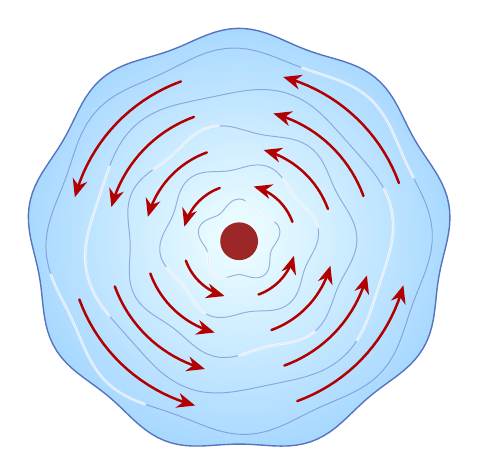
\begin{tikzpicture}[scale=0.8, line cap=round, line join=round]
  \colorlet{arrowcol}{red!70!black}
  \colorlet{spherecol}{cyan!30!blue!90}
  \shade[inner color=cyan!8, outer color=cyan!55!blue!45, opacity=0.75]
    plot[domain=0:360, samples=180, variable=\t]
      ({(3.3+0.08*sin(9*\t))*cos(\t)},{(3.3+0.08*sin(9*\t))*sin(\t)}) -- cycle;
  \draw[spherecol!80, line width=0.5pt, domain=0:360, samples=180, variable=\t]
    plot ({(3.3+0.08*sin(9*\t))*cos(\t)},{(3.3+0.08*sin(9*\t))*sin(\t)});
  \foreach \rr/\kk/\ph/\fa/\fd in {0.6/5/0/30/50, 1.2/6/40/200/45, 1.8/7/80/100/40,
                                  2.4/6/20/150/60, 3.0/8/70/20/50} {%
    \draw[spherecol!70, opacity=0.6, line width=0.35pt, domain=0:360, samples=120, variable=\t]
      plot ({(\rr+0.07*sin(\kk*\t+\ph))*cos(\t)},{(\rr+0.07*sin(\kk*\t+\ph))*sin(\t)});
    \foreach \o in {0,170} {%
      \draw[white, opacity=0.75, line width=0.9pt, domain=\fa+\o:\fa+\o+\fd, samples=25, variable=\t]
        plot ({(\rr+0.07*sin(\kk*\t+\ph))*cos(\t)},{(\rr+0.07*sin(\kk*\t+\ph))*sin(\t)});
    }
  }
  \foreach \rr in {0.9, 1.5, 2.1, 2.7} {%
    \foreach \off in {20, 110, 200, 290} {%
      \draw[-{Stealth[length=2.3mm,width=1.9mm]}, arrowcol, line width=0.9pt,
            domain=\off:\off+55, samples=20, variable=\t]
        plot ({\rr*cos(\t)},{\rr*sin(\t)});
    }
  }
  \fill[red!55!black!85] (0,0) circle (0.3);
\end{tikzpicture}
\end{minipage}

\caption{Shematski prikaz lokalnog vrtložnog gibanja vektorskog polja. Lijevo je prikazana lokalna vrtnja oko osi određene jediničnim vektorom $\overrightarrow{n}$, pri čemu vrijedi $(\operatorname{rot} \overrightarrow{F})\cdot\overrightarrow{n}\neq 0$. Desno je prikazana projekcija tangencijalnih strujnica vrtložnog gibanja na ravninu okomitu na os rotacije.}
\end{figure}

Rotacija opisuje lokalnu vrtložnost vektorskog polja. Može se formalno
zapisati i u determinantnom obliku
$$
\operatorname{rot}\overrightarrow{F}
=
\left|
\begin{array}{ccc}
\overrightarrow{i} & \overrightarrow{j} & \overrightarrow{k} \\[2mm]
\dfrac{\partial}{\partial x} &
\dfrac{\partial}{\partial y} &
\dfrac{\partial}{\partial z} \\[2mm]
F_x & F_y & F_z
\end{array}
\right|.
$$

Gradijent, divergencija i rotacija mogu se zapisati pomoću
diferencijalnog operatora. Oznakom $\nabla$ (nabla) označavamo
\textit{Hamiltonov}\footnote{William Rowan Hamilton (1805.--1865.), irski matematičar i astronom.} diferencijalni operator, koji u Kartezijevim koordinatama formalno zapisujemo kao
$$
\nabla
=
\overrightarrow{i}\frac{\partial}{\partial x}
+
\overrightarrow{j}\frac{\partial}{\partial y}
+
\overrightarrow{k}\frac{\partial}{\partial z}.
$$
Pomoću operatora $\nabla$ prethodno definirani operatori zapisuju se kao
$$
\begin{array}{lcl}
\nabla f & = & \operatorname{grad}f, \\[2mm]
\nabla\cdot\overrightarrow{F} & = & \operatorname{div}\overrightarrow{F}, \\[2mm]
\nabla\times\overrightarrow{F} & = & \operatorname{rot}\overrightarrow{F}.
\end{array}
$$
U nastavku rada koristit ćemo uglavnom zapis pomoću operatora $\nabla$.

\begin{tm}
Neka je $\Omega \subseteq \mathbb{R}^3$ otvoren skup, neka su
$f,g \in C^1(\Omega)$ skalarna polja i
$\overrightarrow{F},\overrightarrow{G} \in C^1(\Omega,\mathbb{R}^3)$ vektorska polja te neka su
$\lambda,\mu \in \mathbb{R}$. Tada vrijedi
\begin{enumerate}
    \item[(i)]
    $
    \nabla(\lambda f+\mu g)
    =
    \lambda\nabla f+\mu\nabla g
    $

    \item[(ii)]
    $
    \nabla\cdot(\lambda\overrightarrow{F}+\mu\overrightarrow{G})
    =
    \lambda(\nabla\cdot\overrightarrow{F})
    +
    \mu(\nabla\cdot\overrightarrow{G})
    $

    \item[(iii)]
    $
    \nabla\times(\lambda\overrightarrow{F}+\mu\overrightarrow{G})
    =
    \lambda(\nabla\times\overrightarrow{F})
    +
    \mu(\nabla\times\overrightarrow{G})
    $

    \item[(iv)]
    $
    \nabla\cdot(f\overrightarrow{F})
    =
    \nabla f\cdot\overrightarrow{F}
    +
    f\,\nabla\cdot\overrightarrow{F}
    $
\end{enumerate}
Svojstva (i), (ii) i (iii) nazivamo svojstvima \textbf{linearnosti} gradijenta,
divergencije i rotacije, dok svojstvo (iv) predstavlja \textbf{Leibnizovo\footnote{Gottfried Wilhelm Leibniz (1646.--1716.), njemački matematičar i filozof.} pravilo},
odnosno pravilo za deriviranje umnoška skalarnog i vektorskog polja.
\end{tm}
\begin{proof}
    Dokaz teorema može se pronaći u \cite{uglesic}.
\end{proof}
\vspace{0.25cm}

\begin{deff}
Vektorsko polje
$\overrightarrow{F}:\Omega\to\mathbb{R}^3$
nazivamo \textbf{\textit{potencijalnim}} ili \textbf{\textit{konzervativnim}} ako postoji
skalarno polje $U:\Omega\to\mathbb{R}$ takvo da je
$\overrightarrow{F}=-\nabla U$. Pritom polje $U$ nazivamo skalarnim
\textbf{\textit{potencijalom}} polja $\overrightarrow{F}$. Za vektorsko polje
$\overrightarrow{F}$ kažemo da je \textbf{\textit{bezvrtložno}} ako je
$\nabla\times\overrightarrow{F}=\overrightarrow{0}$. U protivnom ga nazivamo
\textbf{\textit{vrtložnim}}. Vektorsko polje $\overrightarrow{F}$ nazivamo
\textbf{\textit{solenoidalnim}} ako je $\nabla\cdot\overrightarrow{F}=0$.
\end{deff}
\vspace{0.25cm}

\begin{pr}
Neka je $f(x,y,z)=x^2+y^2+z^2$ skalarno, a 
$\overrightarrow{F}(x,y,z)
=
-y\overrightarrow{i}
+
x\overrightarrow{j}$ vektorsko polje.
Tada vrijedi
$$
\nabla f
= 
\frac{\partial f}{\partial x}\overrightarrow{i}+\frac{\partial f}{\partial y}\overrightarrow{j}+\frac{\partial f}{\partial z}\overrightarrow{k}
=
2x\overrightarrow{i}
+
2y\overrightarrow{j}
+
2z\overrightarrow{k},
$$
dok za polje $\overrightarrow{F}$ vrijedi
$$
\nabla\cdot\overrightarrow{F}=
\frac{\partial F_x}{\partial x}+\frac{\partial F_y}{\partial y}+\frac{\partial F_z}{\partial z}
=
0
$$
i
$$
\nabla\times\overrightarrow{F}=\left|
\begin{array}{ccc}
\overrightarrow{i} & \overrightarrow{j} & \overrightarrow{k} \\[2mm]
\dfrac{\partial}{\partial x} &
\dfrac{\partial}{\partial y} &
\dfrac{\partial}{\partial z} \\[2mm]
F_x & F_y & F_z
\end{array}\right|
=
2\overrightarrow{k}.
$$
Po tome, polje $\overrightarrow{F}$ je solenoidalno, ali nije bezvrtložno. Gradijentno polje $\nabla f$ i solenoidalno vektorsko polje $\overrightarrow{F}$ prikazani su na Slici 4. \end{pr}

\begin{figure}[H]
\centering

\colorlet{polA}{red!75!black}
\colorlet{polB}{blue!75!black}

\def\pivot{0.5}

\def\polje#1#2#3#4#5{%
\resizebox{0.318\textwidth}{!}{%
\begin{tikzpicture}
\begin{axis}[
    width=6cm, height=6cm,
    xmin=-3.1, xmax=3.1, ymin=-3.1, ymax=3.1,
    axis equal image, enlargelimits=false, clip=false,
    axis lines=middle,
    axis line style={->, >={Latex[length=1.8mm,width=1.2mm]},
                     line width=0.55pt, black!65},
    xtick={-3,-2,...,3}, ytick={-3,-2,...,3},
    xticklabels={}, yticklabels={},
    tick style={black!45, line width=0.4pt},
    grid=major, grid style={line width=0.2pt, draw=gray!22},
    title={#5}, title style={font=\small, yshift=-0.5mm}
]

\foreach \ix in {-6,...,6}{
  \foreach \iy in {-6,...,6}{
    \pgfmathsetmacro{\x}{\ix/2}
    \pgfmathsetmacro{\y}{\iy/2}
    \pgfmathsetmacro{\Dx}{#2}
    \pgfmathsetmacro{\Dy}{#3}
    \pgfmathsetmacro{\Q}{sqrt(\Dx*\Dx+\Dy*\Dy)}
    \pgfmathsetmacro{\Nm}{\Q/#4}

    \ifdim\Q pt>0.001pt
      \pgfmathsetmacro{\L}{0.27+0.19*\Nm/(0.25+\Nm)}
      \pgfmathsetmacro{\mix}{32+68*min(1,\Nm/1.2)}
      \pgfmathsetmacro{\lw}{0.5+0.4*min(1,\Nm/1.2)}
      \pgfmathsetmacro{\Ux}{\L*\Dx/\Q}
      \pgfmathsetmacro{\Uy}{\L*\Dy/\Q}
      \pgfmathsetmacro{\Xa}{\x-\pivot*\Ux}
      \pgfmathsetmacro{\Ya}{\y-\pivot*\Uy}
      \pgfmathsetmacro{\Xb}{\x+(1-\pivot)*\Ux}
      \pgfmathsetmacro{\Yb}{\y+(1-\pivot)*\Uy}
      \edef\temp{\noexpand\draw[-{Latex[length=1.15mm,width=0.85mm]},
            color=#1!\mix!white, line width=\lw pt]
        (axis cs:\Xa,\Ya) -- (axis cs:\Xb,\Yb);}%
      \temp
    \else
      \edef\temp{\noexpand\draw[color=#1, fill=white, line width=0.6pt]
        (axis cs:\x,\y) circle (1.7pt);}%
      \temp
    \fi
  }
}


\draw[rounded corners=2pt, black!25]
  (axis description cs:0,0) rectangle (axis description cs:1,1);

\end{axis}
\end{tikzpicture}%
}%
}

\makebox[\textwidth][c]{%
\polje{polA}{2*(\x)}{2*(\y)}{6}{}%
\hspace{0.04\textwidth}%
\polje{polB}{0-(\y)}{(\x)}{3}{}%
}

\captionsetup{justification=centering}
\caption{Vektorska polja $\nabla f$ (lijevo) i $\overrightarrow{F}$ (desno) iz Primjera 2.14., projicirana na ravninu $xy$.}
\end{figure}
\subsection{Laplaceov operator i harmonijske funkcije}

Nakon gradijenta i divergencije prirodno se uvodi operator koji nastaje
njihovim uzastopnim djelovanjem. Taj se operator naziva Laplaceov\footnote{Pierre-Simon Laplace (1749.--1827.), francuski matematičar, astronom i fizičar.} diferencijalni operator.

\begin{deff}
Neka je $f:\Omega\to\mathbb{R}$, $\Omega \subseteq \mathbb{R}^3$ otvoren, skalarno polje klase $C^2$.
\textit{\textbf{Laplaceov} \textbf{diferencijalni operator}} polja $f$
definira se kao divergencija njegova gradijenta
$$
\nabla^2 f
=
\nabla\cdot(\nabla f),
$$
odnosno, u kartezijevim koordinatama
$$
\nabla^2 f
=
\frac{\partial^2 f}{\partial x^2}
+
\frac{\partial^2 f}{\partial y^2}
+
\frac{\partial^2 f}{\partial z^2}.
$$
\end{deff}

Ako je
$
\overrightarrow{F}
=
(F_x,F_y,F_z)
:
\Omega\to\mathbb{R}^3
$
vektorsko polje klase $C^2$, tada Laplaceov operator djeluje na svaku
njegovu komponentu zasebno
$$
\nabla^2\overrightarrow{F}
=
\left(
\nabla^2F_x,
\nabla^2F_y,
\nabla^2F_z
\right).
$$
\begin{tm}
Neka je $\Omega\subseteq\mathbb{R}^3$ otvoren skup i neka je
$f:\Omega\to\mathbb{R}$ skalarno polje klase $C^2$ i
$\overrightarrow{F}:\Omega\to\mathbb{R}^3$ vektorsko polje klase $C^2$.
Tada vrijedi

\begin{enumerate}
    \item[(i)]
    $
    \nabla\times(\nabla f)
    =
    \overrightarrow{0}
    $

    \item[(ii)]
    $
    \nabla\cdot(\nabla\times\overrightarrow{F})
    =
    0
    $

    \item[(iii)]
    $
    \nabla\times(\nabla\times\overrightarrow{F})
    =
    \nabla(\nabla\cdot\overrightarrow{F})
    -
    \nabla^2\overrightarrow{F}
    $
\end{enumerate}
\end{tm}
\begin{proof}
Tvrdnje \textit{(i)} i \textit{(ii)} slijede iz definicija rotacije i divergencije te
\textit{Schwarzova\footnote{Hermann Amandus Schwarz (1843.--1921.), njemački matematičar.} teorema} o jednakosti mješovitih parcijalnih derivacija drugog reda \cite{uglesic},
koji se može primijeniti jer su polja $f$ i $\overrightarrow{F}$ klase $C^2$.
Stoga je dovoljno dokazati tvrdnju \textit{(iii)}. Dvostruku rotaciju vektorskog polja
$\overrightarrow{F}=(F_x,F_y,F_z)$ najprije razvijamo po komponentama. $$
    { \renewcommand{\arraystretch}{1.5}
    \begin{array}{ccc}
\nabla \times (\nabla \times \overrightarrow{F})&=&
\displaystyle\left[
\frac{\partial}{\partial y}
\left(
\frac{\partial F_y}{\partial x}-\frac{\partial F_x}{\partial y}
\right)
-
\frac{\partial}{\partial z}
\left(
\frac{\partial F_x}{\partial z}-\frac{\partial F_z}{\partial x}
\right)
\right]\overrightarrow{i}
\\

&-&
\displaystyle\left[
\frac{\partial}{\partial x}
\left(
\frac{\partial F_y}{\partial x}-\frac{\partial F_x}{\partial y}
\right)
-
\frac{\partial}{\partial z}
\left(
\frac{\partial F_z}{\partial y}-\frac{\partial F_y}{\partial z}
\right)
\right]\overrightarrow{j}
\\

&+&
\displaystyle\left[
\frac{\partial}{\partial x}
\left(
\frac{\partial F_x}{\partial z}-\frac{\partial F_z}{\partial x}
\right)
-
\frac{\partial}{\partial y}
\left(
\frac{\partial F_z}{\partial y}-\frac{\partial F_y}{\partial z}
\right)
\right]\overrightarrow{k}
\\[2em]
&=& \displaystyle \left(
\frac{\partial^2 F_y}{\partial x\partial y}
-\frac{\partial^2 F_x}{\partial y^2}
-\frac{\partial^2 F_x}{\partial z^2}
+\frac{\partial^2 F_z}{\partial x\partial z}
\right)\overrightarrow{i}\\
&+& \displaystyle \left(
\frac{\partial^2 F_x}{\partial x\partial y}-\frac{\partial^2 F_y}{\partial x^2}
+\frac{\partial^2 F_z}{\partial y\partial z}
-\frac{\partial^2 F_y}{\partial z^2}
\right)\overrightarrow{j}\\

&+& \displaystyle \left(
\frac{\partial^2 F_x}{\partial x\partial z}
-\frac{\partial^2 F_z}{\partial x^2}
-\frac{\partial^2 F_z}{\partial y^2}
+\frac{\partial^2 F_y}{\partial y\partial z}
\right)\overrightarrow{k}.\\
\end{array}}
    $$\\ Kako bismo dobivene izraze zapisali pomoću divergencije i Laplaceova operatora, u prvoj komponenti dodajemo i oduzimamo \(\displaystyle \partial^2F_x/\partial x^2\), u drugoj \(\displaystyle \partial^2F_y
    /\partial y^2\), a u trećoj \(\displaystyle \partial^2F_z
    /\partial z^2\). Time dobivamo sljedeće jednakosti.
 $${\renewcommand{\arraystretch}{1.5}
 \begin{array}{ccc}
    \displaystyle
\frac{\partial^2 F_y}{\partial x\partial y}
-\frac{\partial^2 F_x}{\partial y^2}
-\frac{\partial^2 F_x}{\partial z^2}
+\frac{\partial^2 F_z}{\partial x\partial z}
 &=& \displaystyle \frac{\partial}{\partial x}\left( \frac{\partial F_x}{\partial x}+\frac{\partial F_y}{\partial y}+\frac{\partial F_z}{\partial z} \right)-\nabla ^2 F_x, \\
\displaystyle
\frac{\partial^2 F_x}{\partial x\partial y}-\frac{\partial^2 F_y}{\partial x^2}
+\frac{\partial^2 F_z}{\partial y\partial z}
-\frac{\partial^2 F_y}{\partial z^2}
 &=& \displaystyle \frac{\partial}{\partial y}\left( \frac{\partial F_x}{\partial x}+\frac{\partial F_y}{\partial y}+\frac{\partial F_z}{\partial z} \right)-\nabla ^2 F_y,\\

\displaystyle
\frac{\partial^2 F_x}{\partial x\partial z}
-\frac{\partial^2 F_z}{\partial x^2}
-\frac{\partial^2 F_z}{\partial y^2}
+\frac{\partial^2 F_y}{\partial y\partial z}
&=& \displaystyle \frac{\partial}{\partial z}\left( \frac{\partial F_x}{\partial x}+\frac{\partial F_y}{\partial y}+\frac{\partial F_z}{\partial z} \right)-\nabla ^2 F_z. \\[1em]
 \end{array}}
 $$ Uvrštavanjem dobivenih izraza u početnu jednadžbu te primjenom definicija divergencije i Laplaceova operatora za vektorsko polje dobivamo
\[
{\renewcommand{\arraystretch}{1.5}
\begin{array}{ccl}
\nabla \times (\nabla \times \overrightarrow{F})
&=&
\displaystyle
\frac{\partial}{\partial x}
(\nabla\cdot\overrightarrow{F})\overrightarrow{i}
+
\frac{\partial}{\partial y}
(\nabla\cdot\overrightarrow{F})\overrightarrow{j}
+
\frac{\partial}{\partial z}
(\nabla\cdot\overrightarrow{F})\overrightarrow{k}
\\

&-&\displaystyle
\left(
\nabla^2 F_x\,\overrightarrow{i}
+
\nabla^2 F_y\,\overrightarrow{j}
+
\nabla^2 F_z\,\overrightarrow{k}
\right)
\\

&=&
\displaystyle
\nabla(\nabla\cdot\overrightarrow{F})
-
\nabla^2\overrightarrow{F}.
\end{array}}
\]

Time je tvrdnja dokazana.
\end{proof} 
\begin{tm}
Neka je $\Omega\subseteq\mathbb{R}^3$ jednostavno povezano područje i
$\overrightarrow{F}\in C^1(\Omega,\mathbb{R}^3)$. Tada vrijedi
\[
\nabla\times\overrightarrow{F}=\overrightarrow{0}
\quad\Longleftrightarrow\quad
\exists\, U\in C^2(\Omega):
\overrightarrow{F}=-\nabla U.
\]
\end{tm}
\begin{proof}
    Dokaz teorema može se pronaći u \cite{arfken}.
\end{proof}
\begin{deff}
Homogena linearna diferencijalna jednadžba drugog reda oblika
$$
\nabla^2 f=0
$$
naziva se \textbf{\textit{Laplaceova jednadžba}}.
\end{deff}

\begin{deff}
Linearna diferencijalna jednadžba drugog reda oblika
$$
\nabla^2 f=\varphi,
$$
gdje je $\varphi$ zadano skalarno polje, naziva se
\textbf{\textit{Poissonova}\footnote{Siméon Denis Poisson (1781.--1840.), francuski fizičar i matematičar.} \textbf{jednadžba}}.
\end{deff}

Za vektorska polja Poissonova se jednadžba promatra po komponentama. Ako je
$$
\overrightarrow{F}=(F_x,F_y,F_z),
\qquad
\overrightarrow{\varphi}=(\varphi_x,\varphi_y,\varphi_z),
$$
i vrijedi
$$
\nabla^2\overrightarrow{F}=\overrightarrow{\varphi},
$$
tada dobivamo sljedeći sustav jednadžbi:
$$
\begin{aligned}
\frac{\partial^2F_x}{\partial x^2}
+\frac{\partial^2F_x}{\partial y^2}
+\frac{\partial^2F_x}{\partial z^2}
&=\varphi_x,\\
\frac{\partial^2F_y}{\partial x^2}
+\frac{\partial^2F_y}{\partial y^2}
+\frac{\partial^2F_y}{\partial z^2}
&=\varphi_y,\\
\frac{\partial^2F_z}{\partial x^2}
+\frac{\partial^2F_z}{\partial y^2}
+\frac{\partial^2F_z}{\partial z^2}
&=\varphi_z.
\end{aligned}
$$
\begin{deff}
Skalarno polje $f:\Omega\to\mathbb{R}$ klase $C^2$ naziva se
\textbf{\textit{harmonijskim}} na području $\Omega$ ako zadovoljava Laplaceovu
jednadžbu
$$
\nabla^2 f=0.
$$
\end{deff}

\begin{pr}
Neka je $f(x,y,z)=x^2-y^2$ skalarno polje. Tada vrijedi
$$
\nabla^2 f
=
\frac{\partial^2 f}{\partial x^2}
+
\frac{\partial^2 f}{\partial y^2}
+
\frac{\partial^2 f}{\partial z^2}
=
2-2+0
=
0.
$$
Polje $f$ je harmonijsko. \end{pr}

Jedno od važnih svojstava harmonijskih funkcija na cijelom prostoru $\mathbb{R}^3$
daje sljedeći teorem.

\begin{tm}[\textbf{Liouvilleov\footnote{Joseph Liouville (1809.--1882.), francuski matematičar.} teorem}]
Neka je $f:\mathbb{R}^3\to\mathbb{R}$ harmonijska funkcija.
Ako je $f$ ograničena na cijelom prostoru $\mathbb{R}^3$, onda je
$f$ konstantna.
\end{tm}
\begin{proof}
Dokaz ove tvrdnje može se pronaći u \cite{evans}.
\end{proof}

\subsection{Integralni teoremi vektorske analize}

Uz diferencijalne operatore važnu ulogu u vektorskoj analizi imaju i
integralni teoremi. Oni povezuju ponašanje vektorskog polja unutar
promatranog područja s njegovim ponašanjem na granici tog područja.
Za nastavak rada posebno će biti važni teorem o divergenciji,
Greenov drugi identitet i Stokesov teorem. Prije njihova iskaza definirajmo krivuljni
i plošni integral vektorskog polja.


\begin{deff}
Neka je $\overrightarrow{F}:\Omega\to\mathbb{R}^3$ vektorsko polje,
$\Omega\subseteq\mathbb{R}^3$, i neka je
\[
\overrightarrow{r}(t)
=
\bigl(x(t),y(t),z(t)\bigr),
\quad t\in[a,b],
\]
parametrizacija glatke krivulje $\overset{\curvearrowright}{C}\subseteq\Omega$, usmjerene porastom
parametra $t$. Ako je funkcija
\[
t\longmapsto
\overrightarrow{F}(\overrightarrow{r}(t))
\cdot
\overrightarrow{r}'(t)
\]
integrabilna na intervalu $[a,b]$, onda integral
\[
\int\limits_a^b
\overrightarrow{F}(\overrightarrow{r}(t))
\cdot
\overrightarrow{r}'(t)\,dt
\]
nazivamo \textbf{\textit{krivuljnim integralom vektorskog polja}}
$\overrightarrow{F}$ po usmjerenoj krivulji $\overset{\curvearrowright}{C}$ i označavamo s
\[
\int\limits_{\overset{\curvearrowright}{C}}
\overrightarrow{F}\cdot d\overrightarrow{r}.
\]
\end{deff}


Ako je krivulja $\overset{\curvearrowright}{C}$ zatvorena, krivuljni integral zapisujemo u obliku
$$
\oint\limits_{\overset{\curvearrowright}{C}}
\overrightarrow{F}\cdot d\overrightarrow{r}
$$

i nazivamo ga \textbf{\textit{cirkulacijom}} vektorskog polja $\overrightarrow{F}$
duž krivulje $\overset{\curvearrowright}{C}$.

\begin{deff}
Skup $S\subseteq\mathbb{R}^3$ nazivamo \textbf{\textit{plohom}} ako za svaku
točku $T_0\in S$ postoji otvorena okolina $V\subseteq\mathbb{R}^3$ točke
$T_0$, otvoreni skup $U\subseteq\mathbb{R}^2$ i funkcija
$g:U\to\mathbb{R}$ takvi da
\[
z=g(x,y), \qquad (x,y)\in U
\]
bude presječna jednadžba skupa $S\cap V$. Ploha $S$ je
\textbf{\textit{glatka}} ako je pripadna funkcija $g$
diferencijabilna u svakoj točki svoga područja definicije.
\end{deff}

\begin{deff}
Neka je $\overrightarrow{F}=(F_x,F_y,F_z):\Omega\to\mathbb{R}^3$
neprekidno vektorsko polje, a $\overset{\curvearrowright}{S}$ orijentirana glatka ploha zadana
jednadžbom
\[
z=g(x,y), \qquad (x,y)\in D,
\]
gdje je $g:D\to\mathbb{R}$, a $D\subseteq\mathbb{R}^2$ zatvoreno područje
čiji je rub po dijelovima glatka jednostavno zatvorena krivulja. Pri tome neka je odabrana
orijentacija s normalnim vektorom koji ima pozitivnu treću komponentu.
\textbf{\textit{Plošnim integralom vektorskog polja}}
$\overrightarrow{F}$ po plohi $\overset{\curvearrowright}{S}$ nazivamo integral
\[
\iint\limits_D
\left(
-F_x\frac{\partial g}{\partial x}
-F_y\frac{\partial g}{\partial y}
+F_z
\right)
(x,y,g(x,y))\,dx\,dy,
\]
koji označavamo s
\[
\iint\limits_{\overset{\curvearrowright}{S}}
\overrightarrow{F}\cdot d\overrightarrow{S}.
\]
\end{deff}

Plošni integral predstavlja \textbf{\textit{tok}} vektorskog polja $\overrightarrow{F}$ kroz
usmjerenu plohu $\overset{\curvearrowright}{S}$.

\subsubsection{Teorem o divergenciji}

Teorem o divergenciji povezuje divergenciju vektorskog polja unutar
prostornog područja s tokom tog polja kroz njegovu granicu.

\begin{tm}[\textbf{Teorem o divergenciji}]
Neka je $V\subseteq\mathbb{R}^3$ omeđeno područje čija je granica
$\overset{\curvearrowright}{S}=\overset{\curvearrowright}{\partial V}$ zatvorena, po dijelovima glatka ploha orijentirana
vanjskim normalama. Neka je $\overrightarrow{F}$ vektorsko polje klase $C^1$
definirano na području koje sadrži $V$ i njegovu granicu. Tada vrijedi
$$
\iiint\limits_V
\nabla\cdot\overrightarrow{F}\,d\tau
=
\iint\limits_{\overset{\curvearrowright}{S}}
\overrightarrow{F}\cdot d\overrightarrow{S}.
$$
\end{tm}
\begin{proof}
Dokaz ove tvrdnje može se pronaći u \cite{uglesic}.
\end{proof}

\subsubsection{Greenov drugi identitet}

U nastavku donosimo iskaz i dokaz Greenovog drugog identiteta, koji se kasnije u radu koristi za dokaz Helmholtzovog teorema.

\begin{tm}[\textbf{Greenov\footnote{George Green (1793.--1841.), engleski matematičar.} drugi identitet}]
Neka je $V\subseteq\mathbb{R}^3$ omeđeno područje čija je granica
$\overset{\curvearrowright}{S}=\overset{\curvearrowright}{\partial V}$ zatvorena, po dijelovima glatka ploha orijentirana
vanjskim normalama te neka su $f,g:V\to\mathbb{R}$ skalarna polja klase
$C^2$. Tada vrijedi
$$
\iiint\limits_V
\left(
f\nabla^2g-g\nabla^2f
\right)\,d\tau
=
\iint\limits_{\overset{\curvearrowright}{S}}
\left(
f\frac{\partial g}{\partial \overrightarrow{n}}
-
g\frac{\partial f}{\partial \overrightarrow{n}}
\right)\,dS.
$$
\end{tm}

\begin{proof}
Dokaz ove tvrdnje može se pronaći u \cite{daners}.
\end{proof}


\subsubsection{Stokesov teorem}

Stokesov\footnote{George Gabriel Stokes (1819.--1903.), irski matematičar i fizičar.} teorem povezuje cirkulaciju vektorskog polja duž ruba plohe
s tokom njegove rotacije kroz tu plohu.

\begin{deff}
Neka je $\overset{\curvearrowright}{S}$ orijentirana glatka ploha s rubom $\overset{\curvearrowright}{\partial S}$ i neka je
$\overrightarrow{n}$ odabrani jedinični normalni vektor na plohu $\overset{\curvearrowright}{S}$.
Kažemo da su ploha $\overset{\curvearrowright}{S}$ i njezin rub $\overset{\curvearrowright}{\partial S}$
\textbf{\textit{sukladno orijentirani}} ako je orijentacija ruba
$\overset{\curvearrowright}{\partial S}$ određena odabranom orijentacijom plohe $\overset{\curvearrowright}{S}$ po pravilu
desne ruke, pri čemu smjer normalnog vektora $\overrightarrow{n}$
određuje pozitivni smjer obilaska ruba $\overset{\curvearrowright}{\partial S}$.
Promjenom orijentacije plohe $\overset{\curvearrowright}{S}$ mijenja se i odgovarajuća orijentacija
njezina ruba $\overset{\curvearrowright}{\partial S}$.
\end{deff}

\begin{tm}[\textbf{Stokesov teorem}]
Neka je $\overset{\curvearrowright}{S}$ orijentirana, po dijelovima glatka ploha s rubom
$\overset{\curvearrowright}{\partial S}$ i neka je $\overrightarrow{F}$ vektorsko polje klase $C^1$
definirano na području koje sadrži plohu $\overset{\curvearrowright}{S}$. Ako je orijentacija
ruba $\overset{\curvearrowright}{\partial S}$ usklađena s odabranom orijentacijom plohe $\overset{\curvearrowright}{S}$,
onda vrijedi
$$
\int\limits_{\overset{\curvearrowright}{\partial S}}
\overrightarrow{F}\cdot d\overrightarrow{r}
=
\iint\limits_{\overset{\curvearrowright}{S}}
(\nabla\times\overrightarrow{F})\cdot d\overrightarrow{S}.
$$
\end{tm}
\begin{proof}
Dokaz teorema može se pronaći u \cite{uglesic}.
\end{proof}


\subsection{Newtonov potencijal}

Sljedeća lema pokazuje da Newtonov potencijal daje rješenje Poissonove
jednadžbe u \(\mathbb{R}^3\), što će biti ključni korak u dokazu
Helmholtzova teorema.

\begin{lema}
Neka je \(f:\mathbb{R}^3\to\mathbb{R}\) brzo opadajuća funkcija klase
\(C^2\). Definirajmo njezin \textbf{Newtonov\footnote{Isaac Newton (1643.--1727.), engleski matematičar, fizičar i astronom.} potencijal} s
$$
Nf(\overrightarrow{r})
=
\frac{1}{4\pi}
\iiint\limits_{\mathbb{R}^3}
\frac{f(\overrightarrow{r}')}
{\|\overrightarrow{r}-\overrightarrow{r}'\|}\,d\tau'.
$$

Tada je \(Nf\in C^2(\mathbb{R}^3)\) i vrijedi
$$
-\nabla^2Nf=f.
$$
\end{lema}

\begin{proof}
Funkcija
\[
\frac{1}{\left\lVert
\overrightarrow{r}-\overrightarrow{r}'
\right\rVert}
\]
ima singularitet u točki
$\overrightarrow{r}=\overrightarrow{r}'$,
ali je u njemu lokalno integrabilna. Doista, uvedemo li zamjenu
\[
\overrightarrow{x}
=
\overrightarrow{r}-\overrightarrow{r}'
\]
te integral po kugli radijusa $\varepsilon$ zapišemo u sfernim koordinatama, dobivamo
\[
\iiint\limits_{\|\overrightarrow{x}\|<\varepsilon}
\frac{1}{\|\overrightarrow{x}\|}\,dV
=
\int\limits_0^{2\pi}
\int\limits_0^\pi
\int\limits_0^\varepsilon
\frac{1}{\rho}\rho^2\sin\varphi
\,d\rho\,d\varphi\,d\theta.
\]

Stoga
\[
\iiint\limits_{\|\overrightarrow{x}\|<\varepsilon}
\frac{1}{\|\overrightarrow{x}\|}\,dV
=
\int\limits_0^{2\pi} d\theta
\int\limits_0^\pi \sin\varphi\,d\varphi
\int\limits_0^\varepsilon \rho\,d\rho
=
2\pi\varepsilon^2
<
\infty.
\]

Po tome, singularitet u točki
$\overrightarrow{r}=\overrightarrow{r}'$
ne narušava lokalnu integrabilnost integranda, dok konvergencija u beskonačnosti
slijedi iz pretpostavljenog dovoljno brzog opadanja. Stoga je integral
kojim je definiran Newtonov potencijal konačan, odnosno Newtonov je potencijal
dobro definiran.  Uvedimo zamjenu
\[
\overrightarrow{r}'
=
\overrightarrow{r}+\overrightarrow{z}.
\]
Tada je
\[
Nf(\overrightarrow{r})
=
\frac{1}{4\pi}
\iiint\limits_{\mathbb{R}^3}
\frac{f(\overrightarrow{r}+\overrightarrow{z})}
{\|\overrightarrow{z}\|}\,d\tau.
\]
Singularni faktor \(1/\|\overrightarrow{z}\|\) više ne ovisi o
\(\overrightarrow{r}\), pa uz navedene pretpostavke možemo derivirati pod
znakom integrala i dobiti
\[
\nabla^2Nf(\overrightarrow{r})
=
\frac{1}{4\pi}
\iiint\limits_{\mathbb{R}^3}
\frac{\nabla^2f(\overrightarrow{r}+\overrightarrow{z})}
{\|\overrightarrow{z}\|}\,d\tau.
\]
Za fiksnu točku \(\overrightarrow{r}\) stavimo
\[
g(\overrightarrow{z})
=
f(\overrightarrow{r}+\overrightarrow{z}),
\qquad
h(\overrightarrow{z})
=
\frac{1}{\|\overrightarrow{z}\|}.
\]
Promotrimo područje
\[
D_{\varepsilon,R}
=
\{\overrightarrow{z}\in\mathbb{R}^3:
\varepsilon<\|\overrightarrow{z}\|<R\}.
\]
Na tom području funkcija \(h\) je harmonijska, odnosno
\[
\nabla^2h=0.
\]
Primjenom Greenova drugog identiteta dobivamo
\[
\iiint\limits_{D_{\varepsilon,R}}
\left(
h\nabla^2g-g\nabla^2h
\right)d\tau
=
\iint\limits_{\overset{\curvearrowright}{\partial D_{\varepsilon,R}}}
\left(
h\frac{\partial g}{\partial \overrightarrow{n}}
-
g\frac{\partial h}{\partial \overrightarrow{n}}
\right)d\overrightarrow{S}.
\]

Budući da je \(\nabla^2h=0\), slijedi
\[
\iiint\limits_{D_{\varepsilon,R}}
\frac{\nabla^2g(\overrightarrow{z})}
{\|\overrightarrow{z}\|}\,d\tau
=
\iint\limits_{\overset{\curvearrowright}{\partial D_{\varepsilon,R}}}
\left(
\frac{1}{\|\overrightarrow{z}\|}
\frac{\partial g}{\partial \overrightarrow{n}}
-
g\frac{\partial}{\partial \overrightarrow{n}}
\frac{1}{\|\overrightarrow{z}\|}
\right)d\overrightarrow{S}.
\]
Zbog pretpostavljenog opadanja funkcije \(f\) i njezinih derivacija, doprinos
vanjske sfere iščezava kada \(R\to\infty\). Na unutarnjoj sferi
\(\|\overrightarrow{z}\|=\varepsilon\) vanjska normala područja
\(D_{\varepsilon,R}\) usmjerena je prema ishodištu. Zato vrijedi
\[
\frac{\partial g}{\partial \overrightarrow{n}}
=
-\frac{\partial g}{\partial \rho},
\qquad
\frac{\partial h}{\partial \overrightarrow{n}}
=
\frac{1}{\varepsilon^2}.
\]
Dobivamo
\[
\iiint\limits_{D_{\varepsilon,R}}
\frac{\nabla^2g(\overrightarrow{z})}
{\|\overrightarrow{z}\|}\,d\tau
=
-\frac{1}{\varepsilon}
\iint\limits_{\overset{\curvearrowright}{\|\overrightarrow{z}\|=\varepsilon}}
\frac{\partial g}{\partial\rho}\,d\overrightarrow{S}
-
\frac{1}{\varepsilon^2}
\iint\limits_{\overset{\curvearrowright}{\|\overrightarrow{z}\|=\varepsilon}}
g(\overrightarrow{z})\,d\overrightarrow{S}
+o(1).
\]
gdje \(o(1)\to0\) kada \(R\to\infty\). Prvi član s desne strane teži nuli kada \(\varepsilon\to0\). Naime, za prvi član vrijedi
\[
\begin{aligned}
\left|
-\frac{1}{\varepsilon}
\iint\limits_{\overset{\curvearrowright}{\|\overrightarrow{z}\|=\varepsilon}}
\frac{\partial g}{\partial \rho}\,d\overrightarrow{S}
\right|
&\leq
\frac{1}{\varepsilon}
\iint\limits_{\overset{\curvearrowright}{\|\overrightarrow{z}\|=\varepsilon}}
\left|
\frac{\partial g}{\partial \rho}
\right|\,d\overrightarrow{S}
\\
&\leq
\frac{1}{\varepsilon}
\sup\limits_{\|\overrightarrow{z}\|=\varepsilon}
\|\nabla g(\overrightarrow{z})\|
\iint\limits_{\overset{\curvearrowright}{\|\overrightarrow{z}\|=\varepsilon}} d\overrightarrow{S}
\\
&=
\frac{1}{\varepsilon}
\sup\limits_{\|\overrightarrow{z}\|=\varepsilon}
\|\nabla g(\overrightarrow{z})\|
\,4\pi\varepsilon^2
\\
&=
4\pi\varepsilon
\sup\limits_{\|\overrightarrow{z}\|=\varepsilon}
\|\nabla g(\overrightarrow{z})\|,
\end{aligned}
\]
jer
\[
\left|
\frac{\partial g}{\partial \rho}
\right|
=
\left|
\nabla g\cdot\overrightarrow{n}
\right|
\leq
\|\nabla g\|\,\|\overrightarrow{n}\|
=
\|\nabla g\|.
\]

Za drugi član, uz zamjenu
\(\overrightarrow{z}=\varepsilon\overrightarrow{z_0}\), dobivamo
\[
\frac{1}{\varepsilon^2}
\iint\limits_{\overset{\curvearrowright}{\|\overrightarrow{z}\|=\varepsilon}}
g(\overrightarrow{z})\,d\overrightarrow{S}
=
\iint\limits_{\overset{\curvearrowright}{S^2}}
g(\varepsilon\overrightarrow{z_0})\,d\overrightarrow{S}_{\overrightarrow{z_0}}
\longrightarrow
4\pi g(\overrightarrow{0})
=
4\pi f(\overrightarrow{r}),
\]
kada $\varepsilon \to 0$, jer je funkcija $g$ neprekidna u ishodištu.
Po tome,
\[
\iiint\limits_{\mathbb{R}^3}
\frac{\nabla^2f(\overrightarrow{r}+\overrightarrow{z})}
{\|\overrightarrow{z}\|}\,d\tau
=
-4\pi f(\overrightarrow{r}),
\]
pa slijedi
\[
\nabla^2Nf(\overrightarrow{r})
=
-f(\overrightarrow{r}),
\]
odnosno
\[
-\nabla^2Nf=f.
\]
Time je lema dokazana.
\end{proof}

\section{Helmholtzova dekompozicija}
Helmholtzov teorem daje važan rezultat o određivanju vektorskog polja na temelju njegove divergencije i rotacije. Uz odgovarajuće uvjete, vektorsko polje u $\mathbb{R}^3$ može se prikazati kao zbroj gradijenta skalarnog potencijala i rotacije vektorskog potencijala.
\subsection{Helmholtzov teorem}

\begin{tm}[\textbf{Helmholtzov teorem}]
     Neka je \(\overrightarrow{F}:\mathbb{R}^3\to\mathbb{R}^3\) brzo opadajuće vektorsko polje klase \(C^2\). Tada se \(\overrightarrow{F}\) može zapisati u obliku
$$ \overrightarrow{F}=-\nabla U+\nabla\times\overrightarrow{W}, $$
gdje su
$$ U(\overrightarrow{r}) = \frac1{4\pi}\iiint\limits_{\mathbb{R}^3} \frac{\nabla'\cdot\overrightarrow{F}(\overrightarrow{r}')} {\|\overrightarrow{r}-\overrightarrow{r}'\|}\,d\tau' $$
i
$$ \overrightarrow{W}(\overrightarrow{r}) = \frac1{4\pi}\iiint\limits_{\mathbb{R}^3} \frac{\nabla'\times\overrightarrow{F}(\overrightarrow{r}')} {\|\overrightarrow{r}-\overrightarrow{r}'\|}\,d\tau'. $$\\
Prvi član dekompozicije je bezvrtložan, a drugi solenoidalan.
\end{tm}


\begin{proof} 
Definirajmo pomoćno vektorsko polje

$$ \overrightarrow{V}(\overrightarrow{r}) = \frac{1}{4\pi} \iiint\limits_{\mathbb{R}^3} \frac{\overrightarrow{F}(\overrightarrow{r}')} {\|\overrightarrow{r}-\overrightarrow{r}'\|}\,d\tau', $$

pri čemu se integral računa po komponentama. Budući da je \(\overrightarrow{F}\) brzo opadajuće polje klase \(C^2\), svaka njegova komponenta zadovoljava pretpostavke Leme 2.30. Primjenom leme na svaku komponentu polja \(\overrightarrow{F}\) dobivamo
$$ -\nabla^2\overrightarrow{V}=\overrightarrow{F}, $$

gdje Laplaceov operator djeluje po komponentama. Za vektorsko polje \(\overrightarrow{V}\) vrijedi identitet
$$ \nabla\times(\nabla\times\overrightarrow{V}) = \nabla(\nabla\cdot\overrightarrow{V})-\nabla^2\overrightarrow{V}. $$

Po tome,
$$ -\nabla^2\overrightarrow{V} = -\nabla(\nabla\cdot\overrightarrow{V}) + \nabla\times(\nabla\times\overrightarrow{V}). $$\\
Budući da je \(-\nabla^2\overrightarrow{V}=\overrightarrow{F}\), slijedi
$$ \overrightarrow{F} = -\nabla(\nabla\cdot\overrightarrow{V}) + \nabla\times(\nabla\times\overrightarrow{V}). $$

Definiramo
$$ U=\nabla\cdot\overrightarrow{V}, \qquad \overrightarrow{W}=\nabla\times\overrightarrow{V}. $$

Tada dobivamo traženu dekompoziciju
$$  \overrightarrow{F}=-\nabla U+\nabla\times\overrightarrow{W}.  $$

Preostaje pokazati integralne izraze za potencijale \(U\) i \(\overrightarrow{W}\). U izrazu za \(\overrightarrow{V}\) uvedimo zamjenu
$$ \overrightarrow{r}'=\overrightarrow{r}+\overrightarrow{z}. $$

Tada je
$$ \overrightarrow{V}(\overrightarrow{r}) = \frac{1}{4\pi} \iiint\limits_{\mathbb{R}^3} \frac{\overrightarrow{F}(\overrightarrow{r}+\overrightarrow{z})} {\|\overrightarrow{z}\|}\,d\tau. $$

Singularni faktor \(1/\|\overrightarrow{z}\|\) ne ovisi o \(\overrightarrow{r}\), pa zbog glatkoće i brzog opadanja polja \(\overrightarrow{F}\) možemo derivirati pod znakom integrala, kao u dokazu prethodne leme. Stoga

$$ \begin{aligned} U(\overrightarrow{r}) &=\nabla\cdot\overrightarrow{V}(\overrightarrow{r})\\ &= \frac{1}{4\pi} \iiint\limits_{\mathbb{R}^3} \frac{(\nabla\cdot\overrightarrow{F})(\overrightarrow{r}+\overrightarrow{z})} {\|\overrightarrow{z}\|}\,d\tau. \end{aligned} $$

Vraćanjem na varijablu \(\overrightarrow{r}'\) dobivamo
$$  U(\overrightarrow{r}) = \frac{1}{4\pi} \iiint\limits_{\mathbb{R}^3} \frac{\nabla'\cdot\overrightarrow{F}(\overrightarrow{r}')} {\|\overrightarrow{r}-\overrightarrow{r}'\|}\,d\tau'.  $$

Na isti način,
$$ \begin{aligned} \overrightarrow{W}(\overrightarrow{r}) &=\nabla\times\overrightarrow{V}(\overrightarrow{r})\\ &= \frac{1}{4\pi} \iiint\limits_{\mathbb{R}^3} \frac{(\nabla\times\overrightarrow{F})(\overrightarrow{r}+\overrightarrow{z})} {\|\overrightarrow{z}\|}\,d\tau, \end{aligned} $$\\
pa nakon povratka na varijablu \(\overrightarrow{r}'\) slijedi

$$  \overrightarrow{W}(\overrightarrow{r}) = \frac{1}{4\pi} \iiint\limits_{\mathbb{R}^3} \frac{\nabla'\times\overrightarrow{F}(\overrightarrow{r}')} {\|\overrightarrow{r}-\overrightarrow{r}'\|}\,d\tau'.  $$

Konačno,
$$ \nabla\times(-\nabla U)=\overrightarrow{0}, $$

pa je prvi član dekompozicije bezvrtložan, dok je
$$ \nabla\cdot(\nabla\times\overrightarrow{W})=0, $$

pa je drugi član solenoidalan. Time je dokazana Helmholtzova dekompozicija. \end{proof}


\begin{tm}[\textbf{Jedinstvenost polja zadanog divergencijom i rotacijom}]
    Neka su $ \overrightarrow{F}_1,\overrightarrow{F}_2:\mathbb{R}^3\to\mathbb{R}^3 $ vektorska polja klase \(C^2\) takva da vrijedi
$$ \nabla\cdot\overrightarrow{F}_1=\nabla\cdot\overrightarrow{F}_2,\quad \nabla\times\overrightarrow{F}_1=\nabla\times\overrightarrow{F}_2. $$
Pretpostavimo još da 
$$ \overrightarrow{F}_1(\overrightarrow{r})\to \overrightarrow{0}, \qquad \overrightarrow{F}_2(\overrightarrow{r})\to \overrightarrow{0} $$
kada \(\|\overrightarrow{r}\|\to\infty\). Tada je 
\[ \overrightarrow{F}_1=\overrightarrow{F}_2. \]
\end{tm}

\begin{proof}
     Stavimo
$$ \overrightarrow{G}=\overrightarrow{F}_1-\overrightarrow{F}_2. $$
Tada iz pretpostavki i linearnosti operatora $\nabla$ slijedi
$$ \nabla\cdot\overrightarrow{G}=0 $$
i
$$ \nabla\times\overrightarrow{G}=\overrightarrow{0}. $$
Za vektorsko polje \(\overrightarrow{G}\) vrijedi identitet
$$ \nabla^2\overrightarrow{G} = \nabla(\nabla\cdot\overrightarrow{G}) - \nabla\times(\nabla\times\overrightarrow{G}). $$
Zbog
$$ \nabla\cdot\overrightarrow{G}=0, \qquad \nabla\times\overrightarrow{G}=\overrightarrow{0}, $$
dobivamo
$$ \nabla^2\overrightarrow{G}=0. $$
To znači da je svaka komponenta polja \(\overrightarrow{G}\) harmonijska na cijelom \(\mathbb{R}^3\). Po pretpostavci vrijedi
$$ \overrightarrow{F}_1(\overrightarrow{r})\to\overrightarrow{0} $$
i
$$ \overrightarrow{F}_2(\overrightarrow{r})\to\overrightarrow{0} $$
kada \(\|\overrightarrow{r}\|\to\infty\), odnosno
$$ \overrightarrow{G}(\overrightarrow{r})\to\overrightarrow{0}. $$
Stoga je svaka komponenta polja \(\overrightarrow{G}\) ograničena harmonijska funkcija na \(\mathbb{R}^3\). Po Liouvilleovu teoremu svaka je komponenta konstantna. Budući da teži nuli u beskonačnosti, ta konstanta mora biti nula. Po tome,
$$ \overrightarrow{G}=\overrightarrow{0}, $$
pa je
$$ \overrightarrow{F}_1=\overrightarrow{F}_2. $$
\end{proof}

Dakle, vektorsko polje koje iščezava u beskonačnosti jednoznačno je određeno svojom divergencijom i rotacijom.

\begin{pr}
Neka je
\[
\overrightarrow{F}:\mathbb{R}^3\to\mathbb{R}^3,
\qquad
\overrightarrow{F}(x,y,z)
=
\frac{-2y\overrightarrow{i}+2x\overrightarrow{j}}
{(1+x^2+y^2+z^2)^2}.
\]

Najprije provjerimo osnovna svojstva polja. Polje $\overrightarrow{F}\in C^\infty(\mathbb{R}^3)$ iščezava u beskonačnosti. Za
$r=\sqrt{x^2+y^2+z^2}\to\infty$ polje opada reda $r^{-3}$, dok njegove
derivacije opadaju još brže. Nadalje,
\[
\nabla\cdot\overrightarrow{F}=0,
\]
pa je $\overrightarrow{F}$ solenoidalno polje. Budući da gradijentni dio u ovom slučaju iščezava, za skalarni potencijal
možemo uzeti
\[
U=0,
\]
a za vektorski potencijal odabrati
\[
\overrightarrow{W}(x,y,z)
=
\frac{\overrightarrow{k}}
{1+x^2+y^2+z^2}.
\]

Provjerimo da rotacija odabranog vektorskog potencijala daje upravo zadano
polje. Vrijedi
\[
\begin{array}{lcl}
\nabla\times\overrightarrow{W}
=
\left|
\begin{array}{ccc}
\overrightarrow{i} & \overrightarrow{j} & \overrightarrow{k}\\
\dfrac{\partial}{\partial x} &
\dfrac{\partial}{\partial y} &
\dfrac{\partial}{\partial z}\\
W_x&W_y&W_z
\end{array}
\right|
&=&
\displaystyle
\frac{\partial W_z}{\partial y}\overrightarrow{i}
-\frac{\partial W_z}{\partial x}\overrightarrow{j}
\\[1em]
&=&
\displaystyle
-\frac{2y\overrightarrow{i}}
{(1+x^2+y^2+z^2)^2}
+
\frac{2x\overrightarrow{j}}
{(1+x^2+y^2+z^2)^2}
\\[1em]
&=&
\overrightarrow{F}.
\end{array}
\]

Po tome, Helmholtzova dekompozicija ovog polja sadrži samo solenoidalni
dio, odnosno
\[
\overrightarrow{F}
=
\nabla\times\overrightarrow{W}.
\]
\end{pr}

\begin{pr}

Promotrimo vektorsko polje
\[
\overrightarrow{F}(x,y,z)
=
2e^{-(x^2+y^2+z^2)}
\left(
x(z+1)\overrightarrow{i}
+y(z+1)\overrightarrow{j}
+(z+1-x^2-y^2)\overrightarrow{k}
\right).
\]

Polje $\overrightarrow{F}\in C^\infty(\mathbb{R}^3)$ iščezava u
beskonačnosti, a za
$r=\sqrt{x^2+y^2+z^2}\to\infty$ opada brže od svakog reda $r^{-m}$,
$m>0$. Isto vrijedi i za njegove derivacije. Stoga polje zadovoljava
pretpostavke Helmholtzova teorema.

Njegova divergencija iznosi
\[
\nabla\cdot\overrightarrow{F}
=
2\left(3-2(x^2+y^2+z^2)\right)
e^{-(x^2+y^2+z^2)},
\]
dok je njegova rotacija
\[
\nabla\times\overrightarrow{F}
=
2\left(5-2(x^2+y^2+z^2)\right)
e^{-(x^2+y^2+z^2)}
\left(
-y\overrightarrow{i}+x\overrightarrow{j}
\right).
\]

Iz Helmholtzove dekompozicije
\[
\overrightarrow{F}
=
-\nabla U+\nabla\times\overrightarrow{W}
\]
primjenom divergencije dobivamo
\[
\nabla\cdot\overrightarrow{F}
=
-\nabla^2 U,
\]
jer vrijedi
\[
\nabla\cdot
\left(
\nabla\times\overrightarrow{W}
\right)
=0.
\]
Po tome, skalarni potencijal $U$ mora zadovoljavati
\[
-\nabla^2 U
=
2\left(3-2(x^2+y^2+z^2)\right)
e^{-(x^2+y^2+z^2)}.
\]

Budući da vrijedi
\[
-\nabla^2
\left(
e^{-(x^2+y^2+z^2)}
\right)
=
2\left(3-2(x^2+y^2+z^2)\right)
e^{-(x^2+y^2+z^2)},
\]
uz uvjet iščezavanja u beskonačnosti dobivamo
\[
U(x,y,z)
=
e^{-(x^2+y^2+z^2)}.
\]

Za određivanje vektorskog potencijala primijenimo rotaciju na
Helmholtzovu dekompoziciju. Budući da je
\[
\nabla\times(\nabla U)=\overrightarrow{0},
\]
slijedi
\[
\nabla\times\overrightarrow{F}
=
\nabla\times
\left(
\nabla\times\overrightarrow{W}
\right).
\]
Uz izbor
\[
\nabla\cdot\overrightarrow{W}=0
\]
dobivamo
\[
-\nabla^2\overrightarrow{W}
=
\nabla\times\overrightarrow{F}.
\]
Stoga $\overrightarrow{W}$ zadovoljava
\[
-\nabla^2\overrightarrow{W}
=
2\left(5-2(x^2+y^2+z^2)\right)
e^{-(x^2+y^2+z^2)}
\left(
-y\overrightarrow{i}+x\overrightarrow{j}
\right).
\]

Budući da
\[
\begin{aligned}
-\nabla^2
\left[
e^{-(x^2+y^2+z^2)}
\left(
-y\overrightarrow{i}+x\overrightarrow{j}
\right)
\right]
&=
2\left(5-2(x^2+y^2+z^2)\right)e^{-(x^2+y^2+z^2)}\\
&\quad\cdot
\left(
-y\overrightarrow{i}+x\overrightarrow{j}
\right),
\end{aligned}
\]
jedan odgovarajući vektorski potencijal jest
\[
\overrightarrow{W}(x,y,z)
=
e^{-(x^2+y^2+z^2)}
\left(
-y\overrightarrow{i}+x\overrightarrow{j}
\right).
\]

Za bezvrtložni dio sada dobivamo
\[
-\nabla U
=
2e^{-(x^2+y^2+z^2)}
\left(
x\overrightarrow{i}
+y\overrightarrow{j}
+z\overrightarrow{k}
\right),
\]
dok je solenoidalni dio
\[
\nabla\times\overrightarrow{W}
=
2e^{-(x^2+y^2+z^2)}
\left(
xz\overrightarrow{i}
+yz\overrightarrow{j}
+(1-x^2-y^2)\overrightarrow{k}
\right).
\]

Njihovim zbrojem dobivamo
\[
-\nabla U+\nabla\times\overrightarrow{W}
=
\overrightarrow{F}.
\]

Time su iz zadanog polja $\overrightarrow{F}$ rekonstruirani skalarni
potencijal $U$ i vektorski potencijal $\overrightarrow{W}$ te je dobivena
njegova Helmholtzova dekompozicija. Presjeci bezvrtložnog dijela
$-\nabla U$, solenoidalnog dijela
$\nabla\times\overrightarrow{W}$ i vektorskog polja
$\overrightarrow{F}$ u ravnini $xz$ prikazani su na
Slici~\ref{fig:helmholtz-presjeci}.

\begin{figure}[H]
\centering

\colorlet{polA}{red!75!black}
\colorlet{polB}{blue!75!black}
\colorlet{polC}{black!85}

\def\pivot{0.5}

\def\polje#1#2#3#4{%
\resizebox{0.318\textwidth}{!}{%
\begin{tikzpicture}
\begin{axis}[
    width=6cm, height=6cm,
    xmin=-3.1, xmax=3.1, ymin=-3.1, ymax=3.1,
    axis equal image, enlargelimits=false, clip=false,
    axis lines=middle,
    axis line style={->, >={Latex[length=1.8mm,width=1.2mm]},
                     line width=0.55pt, black!65},
    xtick={-3,-2,...,3}, ytick={-3,-2,...,3},
    xticklabels={}, yticklabels={},
    tick style={black!45, line width=0.4pt},
    grid=major, grid style={line width=0.2pt, draw=gray!22},
    title={#4}, title style={font=\small, yshift=-0.5mm}
]

\foreach \ix in {-6,...,6}{
  \foreach \iz in {-6,...,6}{
    \pgfmathsetmacro{\x}{\ix/2}
    \pgfmathsetmacro{\z}{\iz/2}
    \pgfmathsetmacro{\E}{exp(-(\x*\x+\z*\z))}
    \pgfmathsetmacro{\Dx}{#2}
    \pgfmathsetmacro{\Dz}{#3}
    \pgfmathsetmacro{\Q}{sqrt(\Dx*\Dx+\Dz*\Dz)}
    \pgfmathsetmacro{\Nm}{2*\E*\Q}

    \ifdim\Q pt>0.001pt
      \pgfmathsetmacro{\L}{0.27+0.19*\Nm/(0.25+\Nm)}
      \pgfmathsetmacro{\mix}{32+68*min(1,\Nm/1.2)}
      \pgfmathsetmacro{\lw}{0.5+0.4*min(1,\Nm/1.2)}
      \pgfmathsetmacro{\Ux}{\L*\Dx/\Q}
      \pgfmathsetmacro{\Uz}{\L*\Dz/\Q}
      \pgfmathsetmacro{\Xa}{\x-\pivot*\Ux}
      \pgfmathsetmacro{\Za}{\z-\pivot*\Uz}
      \pgfmathsetmacro{\Xb}{\x+(1-\pivot)*\Ux}
      \pgfmathsetmacro{\Zb}{\z+(1-\pivot)*\Uz}
      \edef\temp{\noexpand\draw[-{Latex[length=1.15mm,width=0.85mm]},
            color=#1!\mix!white, line width=\lw pt]
        (axis cs:\Xa,\Za) -- (axis cs:\Xb,\Zb);}%
      \temp
    \else
      \edef\temp{\noexpand\draw[color=#1, fill=white, line width=0.6pt]
        (axis cs:\x,\z) circle (1.7pt);}%
      \temp
    \fi
  }
}

\node[font=\scriptsize, black!65, anchor=north east] at (axis cs:3.0,-0.08) {$x$};
\node[font=\scriptsize, black!65, anchor=north west] at (axis cs:0.08,3.0) {$z$};

\draw[rounded corners=2pt, black!25]
  (axis description cs:0,0) rectangle (axis description cs:1,1);

\end{axis}
\end{tikzpicture}%
}%
}
\polje{polA}{(\x)}{(\z)}{}%
\hfill
\polje{polB}{(\x)*(\z)}{1-(\x)*(\x)}{}%
\hfill
\polje{polC}{(\x)*((\z)+1)}{(\z)+1-(\x)*(\x)}{}

\captionsetup{justification=centering}
\caption{Presjeci polja $-\nabla U$, $\nabla\times\overrightarrow{W}$ i
$\overrightarrow{F}$ iz Primjera 3.4., prikazani redom u ravnini $xz$.}
\end{figure}
\end{pr}

\subsection{Primjene Helmholtzova teorema}
U nastavku navodimo nekoliko klasičnih fizikalnih primjera koji ilustriraju
gradijentnu i solenoidalnu strukturu Helmholtzove dekompozicije. Neki od
navedenih idealiziranih modela, poput polja točkastog naboja ili gravitacijskog polja točkaste mase,
ne zadovoljavaju sve pretpostavke prethodno dokazane verzije Helmholtzova
teorema, ali zorno prikazuju osnovnu strukturu potencijalnih i solenoidalnih
polja. U pojedinim primjerima za skalarni i vektorski potencijal koristit ćemo
oznake uobičajene u odgovarajućem fizikalnom području, umjesto oznaka $U$ i
$\overrightarrow{W}$ iz Helmholtzova teorema.

\subsubsection{Električno polje}
U elektrostatici je električno polje $\overrightarrow{E}$ određeno raspodjelom
električnog naboja. Budući da vrijedi
$$
\nabla\times\overrightarrow{E}=\overrightarrow{0},
$$
električno je polje bezvrtložno pa se može zapisati pomoću skalarnog
potencijala $V$ u obliku
$$
\overrightarrow{E}=-\nabla V.
$$

Po tome, u Helmholtzovoj dekompoziciji električnog polja
solenoidalni dio iščezava, pa ostaje samo gradijentni dio. Primijenimo li divergenciju na prethodnu jednakost i iskoristimo Gaussov\footnote{Carl Friedrich Gauss (1777.--1855.), njemački matematičar, astronom i fizičar.}
zakon
$$
\nabla\cdot\overrightarrow{E}=\frac{\rho}{\varepsilon_0},
$$
gdje je $\rho=\rho(\overrightarrow{r})$ volumna gustoća električnog naboja u promatranoj točki, a $\varepsilon_0$ permitivnost vakuuma, dobivamo
$$
\nabla^2V=-\frac{\rho}{\varepsilon_0}.
$$
Dobivena jednadžba naziva se Poissonova jednadžba za elektrostatski
potencijal.

Za lokaliziranu kontinuiranu raspodjelu naboja s volumnom gustoćom naboja
$\rho(\overrightarrow{r}')$ odgovarajući je potencijal
$$
V(\overrightarrow{r})
=
\frac{1}{4\pi\varepsilon_0}
\iiint\limits_{\mathbb{R}^3}
\frac{\rho(\overrightarrow{r}')}
{\|\overrightarrow{r}-\overrightarrow{r}'\|}
\,d\tau'.
$$

Promotrimo pozitivan točkasti naboj $Q>0$ smješten u ishodištu. U teoriji distribucija takav se naboj opisuje gustoćom
\[
\rho(\overrightarrow{r}) = Q\delta(\overrightarrow{r}),
\]
gdje je $\delta$ Diracova delta-distribucija. Njegovo je električno
polje za $r>0$ dano izrazom
$$
\overrightarrow{E}(\overrightarrow{r})
=
\frac{1}{4\pi\varepsilon_0}
\frac{Q}{r^2}\overrightarrow{r_0},
$$
gdje je $\overrightarrow{r_0}=\displaystyle \frac{\overrightarrow{r}}{r}$ jedinični vektor. Odaberemo li vrijednost potencijala tako da $V(\overrightarrow{r}) \to 0$ kada $r \to \infty$, potencijal
točkastog naboja $Q$ iznosi
$$
V(\overrightarrow{r})
=
\frac{1}{4\pi\varepsilon_0}\frac{Q}{r}.
$$
\begin{figure}[H]
    \centering

    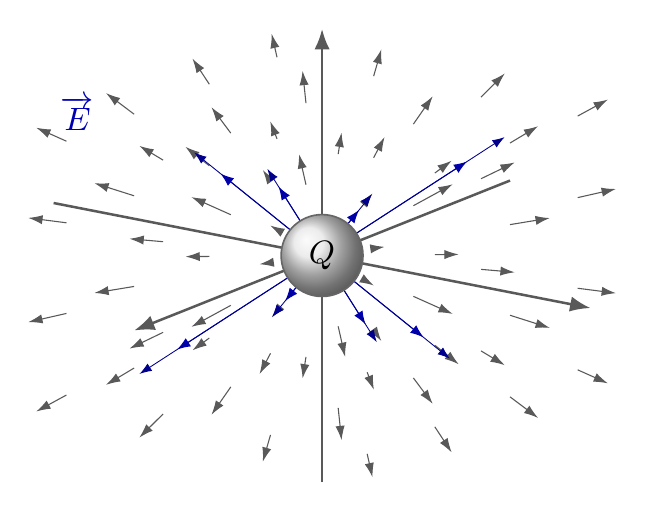
\begin{tikzpicture}[scale=1.3]
        \begin{axis}[
            width=10.5cm,
            height=8.5cm,
            view={125}{22},
            os3d
        ]

        \foreach \x in {-1.4,-0.5,0.5,1.4}{
            \foreach \y in {-1.4,-0.5,0.5,1.4}{
                \foreach \z in {-1.4,-0.5,0.5,1.4}{

                    \pgfmathsetmacro{\rkv}{\x*\x+\y*\y+\z*\z}
                    \pgfmathsetmacro{\r}{sqrt(\rkv)}

                    \pgfmathsetmacro{\Ex}{\x/(\rkv*\r)}
                    \pgfmathsetmacro{\Ey}{\y/(\rkv*\r)}
                    \pgfmathsetmacro{\Ez}{\z/(\rkv*\r)}

                    \pgfmathsetmacro{\Enorma}{sqrt(\Ex*\Ex+\Ey*\Ey+\Ez*\Ez)}

                    \pgfmathsetmacro{\duljina}{0.18 + 0.22*\Enorma/(0.18+\Enorma)}

                    \pgfmathsetmacro{\Xkraj}{\x+\duljina*\Ex/\Enorma}
                    \pgfmathsetmacro{\Ykraj}{\y+\duljina*\Ey/\Enorma}
                    \pgfmathsetmacro{\Zkraj}{\z+\duljina*\Ez/\Enorma}

                    \edef\temp{
                        \noexpand\draw[poljestrelicaMala]
                        (axis cs:\x,\y,\z)
                        --
                        (axis cs:\Xkraj,\Ykraj,\Zkraj);
                    }
                    \temp
                }
            }
        }

        \draw[silnicaplava]
        (axis cs:0.10,0.10,0.10) -- (axis cs:1.15,1.15,1.15);

        \draw[silnicaplava]
        (axis cs:-0.10,-0.10,-0.10) -- (axis cs:-1.15,-1.15,-1.15);

        \draw[silnicaplava]
        (axis cs:0.12,0.12,0) -- (axis cs:1.35,1.35,0);

        \draw[silnicaplava]
        (axis cs:-0.12,-0.12,0) -- (axis cs:-1.35,-1.35,0);

        \draw[silnicaplava]
        (axis cs:0.12,0,0.12) -- (axis cs:1.35,0,1.35);

        \draw[silnicaplava]
        (axis cs:-0.12,0,-0.12) -- (axis cs:-1.35,0,-1.35);

        \draw[silnicaplava]
        (axis cs:0,0.12,0.12) -- (axis cs:0,1.35,1.35);

        \draw[silnicaplava]
        (axis cs:0,-0.12,-0.12) -- (axis cs:0,-1.35,-1.35);

        % vanjske silnice
        \draw[silnicaplavaSlaba]
        (axis cs:0.16,0.16,0.16) -- (axis cs:1.55,1.55,1.55);

        \draw[silnicaplavaSlaba]
        (axis cs:-0.16,-0.16,-0.16) -- (axis cs:-1.55,-1.55,-1.55);

        \draw[silnicaplavaSlaba]
        (axis cs:0.18,0.18,0) -- (axis cs:1.70,1.70,0);

        \draw[silnicaplavaSlaba]
        (axis cs:-0.18,-0.18,0) -- (axis cs:-1.70,-1.70,0);

        \draw[silnicaplavaSlaba]
        (axis cs:0.18,0,0.18) -- (axis cs:1.70,0,1.70);

        \draw[silnicaplavaSlaba]
        (axis cs:-0.18,0,-0.18) -- (axis cs:-1.70,0,-1.70);

        \draw[silnicaplavaSlaba]
        (axis cs:0,0.18,0.18) -- (axis cs:0,1.70,1.70);

        \draw[silnicaplavaSlaba]
        (axis cs:0,-0.18,-0.18) -- (axis cs:0,-1.70,-1.70);

        \shade[
            ball color=gray!20,
            draw=black!60,
            line width=0.45pt
        ]
        (axis cs:0,0,0) circle[radius=4mm];

        \node[
            font=\small
        ]
        at (axis cs:0,0,0) {$Q$};

        \node[
            anchor=west,
            font=\small,
            blue!70!black
        ]
        at (axis description cs:0.2,0.70)
        {$\overrightarrow{E}$};

        \end{axis}

    \end{tikzpicture}

    \caption{Pozitivan točkasti naboj $Q$ u ishodištu i njegovo električno polje.}
\end{figure}

Budući da su električno polje i potencijal singularni u ishodištu, ovaj idealizirani primjer ne zadovoljava izravno pretpostavke prethodno dokazane verzije Helmholtzova teorema.
\subsubsection{Magnetsko polje}

U magnetostatici magnetsko polje $\overrightarrow{B}$ zadovoljava
Ampèreov zakon u diferencijalnom obliku
$$
\nabla\times\overrightarrow{B}=\mu_0\overrightarrow{J},
$$
gdje je $\overrightarrow{J}$ gustoća električne struje, a $\mu_0$
permeabilnost vakuuma.
Primjenom Stokesova teorema dobivamo integralni oblik Ampèreova\footnote{André-Marie Ampère (1775.--1836.), francuski fizičar, matematičar, kemičar i filozof.} zakona
$$
\int\limits_{\overset{\curvearrowright}{C}} \overrightarrow{B}\cdot d\overrightarrow{r}
=
\mu_0\iint\limits_{\overset{\curvearrowright}{S}} \overrightarrow{J}\cdot d\overrightarrow{S},
$$
odnosno
$$
\int\limits_{\overset{\curvearrowright}{C}} \overrightarrow{B}\cdot d\overrightarrow{r}
=
\mu_0 I,
$$
gdje je $I$ ukupna struja koja prolazi kroz plohu omeđenu
krivuljom $\overset{\curvearrowright}{C}$.
\begin{figure}[H]
    \centering

    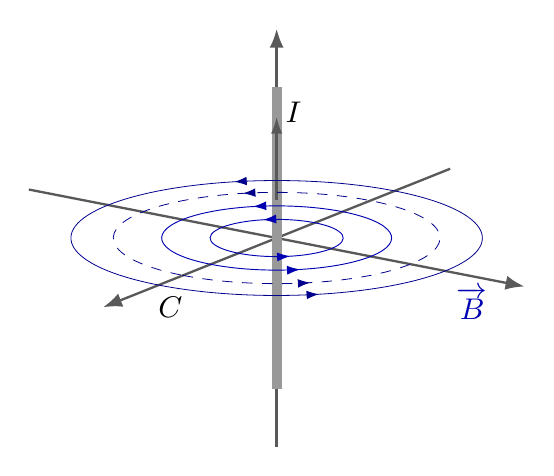
\begin{tikzpicture}[scale=1.2]
        \begin{axis}[
            width=10.5cm,
            height=8.5cm,
            view={125}{22},
            os3d
        ]

        \node[
            anchor=west,
            font=\small,
            blue!70!black
        ]
        at (axis description cs:0.70,0.40)
        {$\overrightarrow{B}$};

        \draw[
            line width=3.0pt,
            black!40
        ]
        (axis cs:0,0,-1.8) --
        (axis cs:0,0,1.8);

        \draw[
            ->,
            >={Latex[length=1.8mm,width=1.2mm]},
            line width=0.70pt,
            black!65
        ]
        (axis cs:0,0,0.45) --
        (axis cs:0,0,1.45);

        \node[
            font=\small,
            anchor=west
        ]
        at (axis cs:0.04,0,1.52) {$I$};

        \draw[
            blue!70!black,
            line width=0.28pt,
            line cap=round,
            line join=round,
            postaction={decorate},
            decoration={
                markings,
                mark=at position 0.18 with {
                    \arrow{Latex[length=1.4mm,width=0.95mm]}
                },
                mark=at position 0.68 with {
                    \arrow{Latex[length=1.4mm,width=0.95mm]}
                }
            }
        ]
        (axis cs:0.55,0,0)
        .. controls (axis cs:0.55,0.304,0)
                    and (axis cs:0.304,0.55,0) ..
        (axis cs:0,0.55,0)
        .. controls (axis cs:-0.304,0.55,0)
                    and (axis cs:-0.55,0.304,0) ..
        (axis cs:-0.55,0,0)
        .. controls (axis cs:-0.55,-0.304,0)
                    and (axis cs:-0.304,-0.55,0) ..
        (axis cs:0,-0.55,0)
        .. controls (axis cs:0.304,-0.55,0)
                    and (axis cs:0.55,-0.304,0) ..
        (axis cs:0.55,0,0);

        \draw[
            blue!70!black,
            line width=0.28pt,
            line cap=round,
            line join=round,
            postaction={decorate},
            decoration={
                markings,
                mark=at position 0.18 with {
                    \arrow{Latex[length=1.4mm,width=0.95mm]}
                },
                mark=at position 0.68 with {
                    \arrow{Latex[length=1.4mm,width=0.95mm]}
                }
            }
        ]
        (axis cs:0.95,0,0)
        .. controls (axis cs:0.95,0.525,0)
                    and (axis cs:0.525,0.95,0) ..
        (axis cs:0,0.95,0)
        .. controls (axis cs:-0.525,0.95,0)
                    and (axis cs:-0.95,0.525,0) ..
        (axis cs:-0.95,0,0)
        .. controls (axis cs:-0.95,-0.525,0)
                    and (axis cs:-0.525,-0.95,0) ..
        (axis cs:0,-0.95,0)
        .. controls (axis cs:0.525,-0.95,0)
                    and (axis cs:0.95,-0.525,0) ..
        (axis cs:0.95,0,0);

        \draw[
            dashed,
            blue!55!black,
            line width=0.24pt,
            line cap=round,
            line join=round,
            postaction={decorate},
            decoration={
                markings,
                mark=at position 0.18 with {
                    \arrow{Latex[length=1.3mm,width=0.9mm]}
                },
                mark=at position 0.68 with {
                    \arrow{Latex[length=1.3mm,width=0.9mm]}
                }
            }
        ]
        (axis cs:1.35,0,0)
        .. controls (axis cs:1.35,0.746,0)
                    and (axis cs:0.746,1.35,0) ..
        (axis cs:0,1.35,0)
        .. controls (axis cs:-0.746,1.35,0)
                    and (axis cs:-1.35,0.746,0) ..
        (axis cs:-1.35,0,0)
        .. controls (axis cs:-1.35,-0.746,0)
                    and (axis cs:-0.746,-1.35,0) ..
        (axis cs:0,-1.35,0)
        .. controls (axis cs:0.746,-1.35,0)
                    and (axis cs:1.35,-0.746,0) ..
        (axis cs:1.35,0,0);

        \draw[
            blue!55!black,
            line width=0.24pt,
            line cap=round,
            line join=round,
            postaction={decorate},
            decoration={
                markings,
                mark=at position 0.18 with {
                    \arrow{Latex[length=1.3mm,width=0.9mm]}
                },
                mark=at position 0.68 with {
                    \arrow{Latex[length=1.3mm,width=0.9mm]}
                }
            }
        ]
        (axis cs:1.70,0,0)
        .. controls (axis cs:1.70,0.939,0)
                    and (axis cs:0.939,1.70,0) ..
        (axis cs:0,1.70,0)
        .. controls (axis cs:-0.939,1.70,0)
                    and (axis cs:-1.70,0.939,0) ..
        (axis cs:-1.70,0,0)
        .. controls (axis cs:-1.70,-0.939,0)
                    and (axis cs:-0.939,-1.70,0) ..
        (axis cs:0,-1.70,0)
        .. controls (axis cs:0.939,-1.70,0)
                    and (axis cs:1.70,-0.939,0) ..
        (axis cs:1.70,0,0);

        \node[
            font=\small,
            anchor=west
        ]
        at (axis cs:2.3,0.3,0) {$C$};

        \end{axis}
    \end{tikzpicture}

    \captionsetup{justification=centering}
    \caption{Silnice magnetskog polja i Ampèreova krivulja $C$
    oko ravnog vodiča kojim prolazi električna struja.}
\end{figure}
Budući da u magnetostatici dodatno vrijedi
$$
\nabla\cdot\overrightarrow{B}=0,
$$
gradijentni dio Helmholtzove dekompozicije polja $\overrightarrow{B}$ jednak je nuli, pa je $\overrightarrow{B}$ potpuno solenoidalno polje.
Zato se može zapisati pomoću vektorskog potencijala $\overrightarrow{A}$ u obliku
$$
\overrightarrow{B}=\nabla\times\overrightarrow{A}.
$$
Budući da je
$$
\nabla\times\overrightarrow{B}=\mu_0\overrightarrow{J},
$$
vektorski se potencijal može odrediti iz odgovarajuće Helmholtzove integralne formule. Iz izraza za vektorski potencijal u Helmholtzovu teoremu dobivamo
$$
\overrightarrow{A}(\overrightarrow{r})
=
\frac{\mu_0}{4\pi}
\iiint\limits_{\mathbb{R}^3}
\frac{\overrightarrow{J}(\overrightarrow{r}')}
{\|\overrightarrow{r}-\overrightarrow{r}'\|}
\,d\tau'.
$$

\subsubsection{Gravitacijsko polje}

Gravitacijsko polje $\overrightarrow{g}$ još je jedan primjer
potencijalnog vektorskog polja. Za njega vrijedi
$$
\nabla\times\overrightarrow{g}=\overrightarrow{0}.
$$
Budući da za gravitacijsko polje vrijedi
$$
\nabla\cdot\overrightarrow{g}=-4\pi G\rho
\qquad
\nabla\times\overrightarrow{g}=\overrightarrow{0},
$$
solenoidalni dio Helmholtzove dekompozicije gravitacijskog polja iščezava te ostaje samo gradijentni dio,
\[
\overrightarrow{g} = -\nabla \Phi.
\]

Primjenom divergencije na ovu jednakost dobivamo Poissonovu jednadžbu za gravitacijski potencijal.
$$
\nabla^2\Phi=4\pi G\rho.
$$

Za kontinuiranu raspodjelu mase s volumnom gustoćom mase
$\rho(\overrightarrow{r}')$ gravitacijski potencijal ima oblik
$$
\Phi(\overrightarrow{r})
=
-G
\iiint\limits_{\mathbb{R}^3}
\frac{\rho(\overrightarrow{r}')}
{\|\overrightarrow{r}-\overrightarrow{r}'\|}
\,d\tau'.
$$

\noindent Za točkastu masu $M$ smještenu u ishodištu gravitacijsko je polje dano
izrazom
$$
\overrightarrow{g}(\overrightarrow{r})
=
-\frac{GM}{r^2}\overrightarrow{r_0},
$$
gdje je $G$ gravitacijska konstanta.
Predznak minus označava da je gravitacijsko polje usmjereno
prema masi $M$.
Odaberemo li vrijednost potencijala koja iščezava u beskonačnosti, gravitacijski
potencijal točkaste mase iznosi
$$
\Phi(\overrightarrow{r})
=
-\frac{GM}{r}.
$$

\begin{figure}[H]
    \centering

    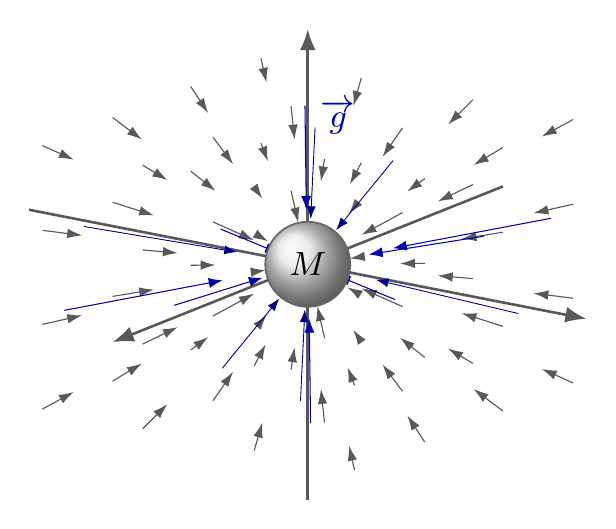
\begin{tikzpicture}[scale=1.35]
        \begin{axis}[
            width=10.5cm,
            height=8.5cm,
            view={125}{22},
            os3d
        ]

        \foreach \x in {-1.4,-0.5,0.5,1.4}{
            \foreach \y in {-1.4,-0.5,0.5,1.4}{
                \foreach \z in {-1.4,-0.5,0.5,1.4}{

                    \pgfmathsetmacro{\rkv}{\x*\x+\y*\y+\z*\z}
                    \pgfmathsetmacro{\r}{sqrt(\rkv)}

                    \pgfmathsetmacro{\gx}{-\x/(\rkv*\r)}
                    \pgfmathsetmacro{\gy}{-\y/(\rkv*\r)}
                    \pgfmathsetmacro{\gz}{-\z/(\rkv*\r)}

                    \pgfmathsetmacro{\gnorma}
                    {sqrt(\gx*\gx+\gy*\gy+\gz*\gz)}

                    \pgfmathsetmacro{\duljina}
                    {0.18 + 0.22*\gnorma/(0.18+\gnorma)}

                    \pgfmathsetmacro{\Xkraj}
                    {\x+\duljina*\gx/\gnorma}

                    \pgfmathsetmacro{\Ykraj}
                    {\y+\duljina*\gy/\gnorma}

                    \pgfmathsetmacro{\Zkraj}
                    {\z+\duljina*\gz/\gnorma}

                    \edef\temp{
                        \noexpand\draw[poljestrelicaMala]
                        (axis cs:\x,\y,\z)
                        --
                        (axis cs:\Xkraj,\Ykraj,\Zkraj);
                    }
                    \temp
                }
            }
        }

        \draw[silnicaplava]
        (axis cs:1.85,0.10,0.20)
        --
        (axis cs:0.62,0.03,0.07);

        \draw[silnicaplava]
        (axis cs:-1.75,0.35,-0.20)
        --
        (axis cs:-0.61,0.12,-0.07);

        \draw[silnicaplava]
        (axis cs:1.10,1.55,0.35)
        --
        (axis cs:0.36,0.51,0.12);

        \draw[silnicaplava]
        (axis cs:-1.10,-1.55,-0.35)
        --
        (axis cs:-0.36,-0.51,-0.12);

        \draw[silnicaplava]
        (axis cs:-0.90,1.55,0.55)
        --
        (axis cs:-0.32,0.54,0.19);

        \draw[silnicaplava]
        (axis cs:0.90,-1.55,-0.55)
        --
        (axis cs:0.32,-0.54,-0.19);

        \draw[silnicaplava]
        (axis cs:0.25,0.15,1.80)
        --
        (axis cs:0.09,0.05,0.62);

        \draw[silnicaplava]
        (axis cs:-0.25,-0.15,-1.80)
        --
        (axis cs:-0.09,-0.05,-0.62);

        \draw[silnicaplavaSlaba]
        (axis cs:1.65,-0.85,0.75)
        --
        (axis cs:0.52,-0.27,0.24);

        \draw[silnicaplavaSlaba]
        (axis cs:-1.55,0.80,-0.85)
        --
        (axis cs:-0.50,0.26,-0.27);

        \draw[silnicaplavaSlaba]
        (axis cs:0.55,1.15,1.55)
        --
        (axis cs:0.18,0.38,0.51);

        % donja
        \draw[silnicaplavaSlaba]
        (axis cs:-0.55,-1.15,-1.55)
        --
        (axis cs:-0.18,-0.38,-0.51);

        \draw[silnicaplavaSlaba]
        (axis cs:-1.45,-0.95,0.75)
        --
        (axis cs:-0.48,-0.31,0.25);

        \draw[silnicaplavaSlaba]
        (axis cs:1.45,0.95,-0.75)
        --
        (axis cs:0.48,0.31,-0.25);

        \shade[
            ball color=gray!20,
            draw=black!60,
            line width=0.45pt
        ]
        (axis cs:0,0,0) circle[radius=4mm];

        \node[
            font=\small
        ]
        at (axis cs:0,0,0) {$M$};

        \node[
            anchor=west,
            font=\small,
            blue!70!black
        ]
        at (axis description cs:0.50,0.70)
        {$\overrightarrow{g}$};

        \end{axis}
    \end{tikzpicture}

    \captionsetup{justification=centering}
    \caption{Točkasta masa $M$ u ishodištu i gravitacijsko polje $\overrightarrow{g}$.}
\end{figure}

Točkasta masa $M$ u ishodištu formalno se opisuje gustoćom
\[
\rho(\overrightarrow{r}) = M\delta(\overrightarrow{r}).
\]
Potencijal $\Phi$ i gravitacijsko polje $\overrightarrow{g}$ singularni su u ishodištu i ne zadovoljavaju izravno pretpostavke iz Helmholtzova teorema.
\subsubsection{Dinamika fluida}

Još jedna primjena Helmholtzove dekompozicije pojavljuje se u dinamici
fluida. Gibanje fluida opisuje se poljem brzine $\overrightarrow{v}=\overrightarrow{v}(\overrightarrow{r})$, koje svakoj
točki prostora pridružuje brzinu čestice fluida u toj točki. Rotacija polja brzine opisuje lokalno vrtložno gibanje fluida.
Ako je strujanje bezvrtložno, tada vrijedi
$$
\nabla\times\overrightarrow{v}=\overrightarrow{0}.
$$
Na jednostavno povezanom području takvo se polje brzine može zapisati pomoću skalarnog potencijala
$\phi$ u obliku
$$
\overrightarrow{v}=-\nabla\phi.
$$
Funkcija $\phi$ naziva se potencijal brzine. Po tome, kod bezvrtložnog strujanja polje brzine predstavlja
gradijentni dio Helmholtzove dekompozicije. Kod nestlačivog strujanja gustoća fluida duž strujanja ostaje konstantna, a za fluid konstantne gustoće jednadžba kontinuiteta daje
\[
\nabla \cdot \overrightarrow{v} = 0.
\]

Tada, uz pretpostavke Helmholtzova teorema, gradijentni dio Helmholtzove dekompozicije iščezava te je polje brzine solenoidalno, pa se može zapisati kao rotacija vektorskog potencijala. Općenito, ako polje brzine zadovoljava pretpostavke Helmholtzova teorema,
može se zapisati u obliku
\[
\overrightarrow{v}
=
-\nabla \phi
+
\nabla\times\overrightarrow{A},
\]
gdje prvi dio opisuje bezvrtložni, a drugi solenoidalni dio polja brzine.

\begin{figure}[H]
\centering
\begin{minipage}[t]{0.48\textwidth}
\vspace{0pt}
\centering

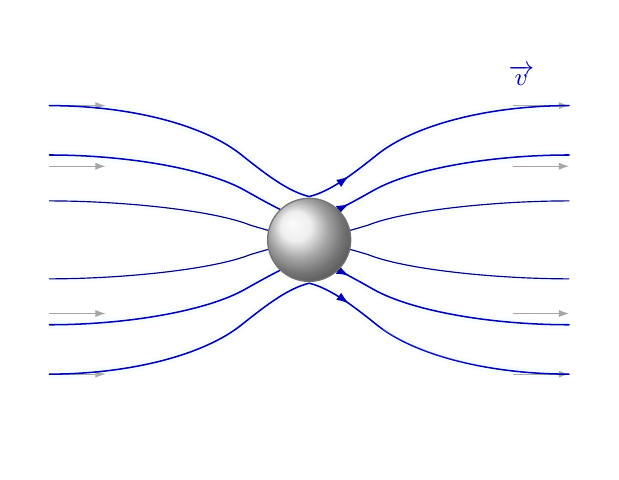
\begin{tikzpicture}[scale=1.1,
    tok/.style={
        preaction={
            draw=cyan!30,
            line width=3.2pt,
            opacity=0.10
        },
        blue!70!black,
        line width=0.55pt,
        line cap=round,
        line join=round,
        postaction={decorate},
        decoration={
            markings,
            mark=at position 0.58 with {
                \arrow{Latex[length=1.6mm,width=1.1mm]}
            }
        }
    },
    tokSlab/.style={
        preaction={
            draw=cyan!25,
            line width=2.6pt,
            opacity=0.08
        },
        blue!50!black,
        line width=0.42pt,
        line cap=round,
        line join=round,
        postaction={decorate},
        decoration={
            markings,
            mark=at position 0.58 with {
                \arrow{Latex[length=1.4mm,width=1.0mm]}
            }
        }
    }
]

\foreach \y in {-1.55,-0.85,0.85,1.55}{
    \draw[
        ->,
        >={Latex[length=1.3mm,width=0.9mm]},
        black!35,
        line width=0.32pt
    ]
    (-3.0,\y) -- (-2.35,\y);

    \draw[
        ->,
        >={Latex[length=1.3mm,width=0.9mm]},
        black!35,
        line width=0.32pt
    ]
    (2.35,\y) -- (3.0,\y);
}

\draw[tok]
(-3,1.55)
.. controls (-2.05,1.55) and (-1.20,1.32) ..
(-0.78,0.98)
.. controls (-0.48,0.74) and (-0.24,0.56) ..
(0,0.50)
.. controls (0.24,0.56) and (0.48,0.74) ..
(0.78,0.98)
.. controls (1.20,1.32) and (2.05,1.55) ..
(3,1.55);

\draw[tok]
(-3,0.98)
.. controls (-2.10,0.98) and (-1.18,0.82) ..
(-0.74,0.57)
.. controls (-0.42,0.39) and (-0.20,0.27) ..
(0,0.22)
.. controls (0.20,0.27) and (0.42,0.39) ..
(0.74,0.57)
.. controls (1.18,0.82) and (2.10,0.98) ..
(3,0.98);

\draw[tokSlab]
(-3,0.45)
.. controls (-2.15,0.45) and (-1.10,0.34) ..
(-0.68,0.17)
.. controls (-0.38,0.08) and (-0.18,0.03) ..
(0,0.015)
.. controls (0.18,0.03) and (0.38,0.08) ..
(0.68,0.17)
.. controls (1.10,0.34) and (2.15,0.45) ..
(3,0.45);

\draw[tokSlab]
(-3,-0.45)
.. controls (-2.15,-0.45) and (-1.10,-0.34) ..
(-0.68,-0.17)
.. controls (-0.38,-0.08) and (-0.18,-0.03) ..
(0,-0.015)
.. controls (0.18,-0.03) and (0.38,-0.08) ..
(0.68,-0.17)
.. controls (1.10,-0.34) and (2.15,-0.45) ..
(3,-0.45);

\draw[tok]
(-3,-0.98)
.. controls (-2.10,-0.98) and (-1.18,-0.82) ..
(-0.74,-0.57)
.. controls (-0.42,-0.39) and (-0.20,-0.27) ..
(0,-0.22)
.. controls (0.20,-0.27) and (0.42,-0.39) ..
(0.74,-0.57)
.. controls (1.18,-0.82) and (2.10,-0.98) ..
(3,-0.98);

\draw[tok]
(-3,-1.55)
.. controls (-2.05,-1.55) and (-1.20,-1.32) ..
(-0.78,-0.98)
.. controls (-0.48,-0.74) and (-0.24,-0.56) ..
(0,-0.50)
.. controls (0.24,-0.56) and (0.48,-0.74) ..
(0.78,-0.98)
.. controls (1.20,-1.32) and (2.05,-1.55) ..
(3,-1.55);

\draw[
    white,
    opacity=0.28,
    line width=0.35pt,
    line cap=round
]
(-2.7,1.60)
.. controls (-2.0,1.60) and (-1.45,1.48) ..
(-1.08,1.29);

\draw[
    cyan!15!white,
    opacity=0.30,
    line width=0.30pt,
    line cap=round
]
(0.85,-1.03)
.. controls (1.35,-1.35) and (2.0,-1.50) ..
(2.65,-1.50);

\shade[
    ball color=gray!18,
    draw=black!55,
    line width=0.45pt
]
(0,0) circle (0.48);

\node[
    blue!70!black,
    font=\small
]
at (2.45,1.90)
{$\overrightarrow{v}$};
\pgfresetboundingbox
\path[use as bounding box] (-3.25,-2.45) rectangle (3.25,2.45);
\end{tikzpicture}

\end{minipage}
\hfill

\begin{minipage}[t]{0.48\textwidth}
\vspace{0pt}
\centering

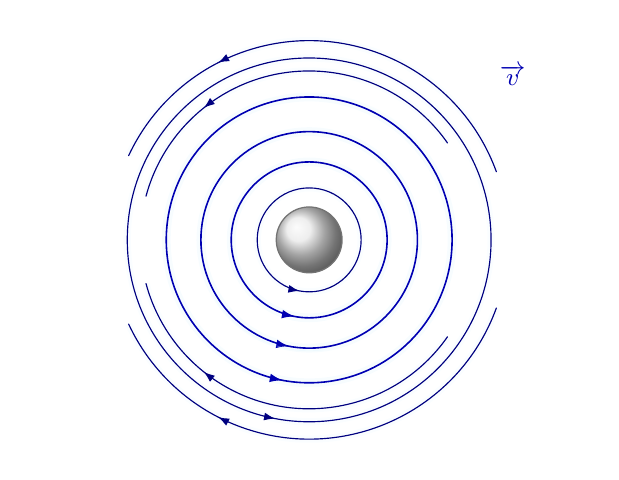
\begin{tikzpicture}[scale=1.1,
    vrtlog/.style={
        preaction={
            draw=cyan!30,
            line width=3.2pt,
            opacity=0.10
        },
        blue!70!black,
        line width=0.58pt,
        line cap=round,
        line join=round,
        postaction={decorate},
        decoration={
            markings,
            mark=at position 0.72 with {
                \arrow{Latex[length=1.6mm,width=1.1mm]}
            }
        }
    },
    vrtlogSlab/.style={
        preaction={
            draw=cyan!25,
            line width=2.6pt,
            opacity=0.08
        },
        blue!50!black,
        line width=0.42pt,
        line cap=round,
        line join=round,
        postaction={decorate},
        decoration={
            markings,
            mark=at position 0.72 with {
                \arrow{Latex[length=1.4mm,width=1.0mm]}
            }
        }
    }
]

\draw[vrtlogSlab]
(0,0) circle (2.10);

\draw[vrtlog]
(0,0) circle (1.65);

\draw[vrtlog]
(0,0) circle (1.25);

\draw[vrtlog]
(0,0) circle (0.90);

\draw[vrtlogSlab]
(0,0) circle (0.60);

\draw[vrtlogSlab]
(20:2.30)
arc[
    start angle=20,
    end angle=155,
    radius=2.30
];

\draw[vrtlogSlab]
(-20:2.30)
arc[
    start angle=-20,
    end angle=-155,
    radius=2.30
];

\draw[vrtlogSlab]
(35:1.95)
arc[
    start angle=35,
    end angle=165,
    radius=1.95
];

\draw[vrtlogSlab]
(-35:1.95)
arc[
    start angle=-35,
    end angle=-165,
    radius=1.95
];

\draw[
    white,
    opacity=0.30,
    line width=0.35pt,
    line cap=round
]
(35:1.70)
arc[
    start angle=35,
    end angle=105,
    radius=1.70
];

\draw[
    cyan!15!white,
    opacity=0.30,
    line width=0.30pt,
    line cap=round
]
(210:1.28)
arc[
    start angle=210,
    end angle=278,
    radius=1.28
];

\shade[
    ball color=gray!18,
    draw=black!55,
    line width=0.45pt
]
(0,0) circle (0.38);

\node[
    blue!70!black,
    font=\small
]
at (2.35,1.90)
{$\overrightarrow{v}$};
\pgfresetboundingbox
\path[use as bounding box] (-3.25,-2.45) rectangle (3.25,2.45);
\end{tikzpicture}

\end{minipage}

\captionsetup{justification=centering}
\caption{Shematski prikaz dviju vrsta strujanja fluida: lijevo je prikazano
bezvrtložno, a desno vrtložno strujanje.}
\end{figure} \newpage
\section{Zaključak}

U ovom radu razmatrana je Helmholtzova dekompozicija glatkih i brzo
opadajućih vektorskih polja u prostoru $\mathbb{R}^3$. U tu su svrhu
prikazani pojmovi i rezultati vektorske analize potrebni za formulaciju i
dokaz glavnog rezultata, među kojima su gradijent, divergencija, rotacija,
Laplaceov operator, harmonijske funkcije i integralni teoremi vektorske
analize. Posebna je pozornost posvećena Newtonovu potencijalu i njegovoj
povezanosti s Poissonovom jednadžbom.

Središnji rezultat rada predstavlja Helmholtzov teorem, po kojem se,
uz odgovarajuće uvjete glatkoće i opadanja u beskonačnosti, vektorsko polje
$\overrightarrow{F}$ može zapisati u obliku
\[
\overrightarrow{F}
=
-\nabla U
+
\nabla\times\overrightarrow{W},
\]
gdje je $U$ skalarni, a $\overrightarrow{W}$ vektorski potencijal. Na taj se
način vektorsko polje rastavlja na bezvrtložni i solenoidalni dio. Izvedeni su
integralni izrazi za pripadne potencijale te je pokazano da je, uz zadane
uvjete u beskonačnosti, vektorsko polje jednoznačno određeno svojom
divergencijom i rotacijom.

Struktura dekompozicije dodatno je prikazana na dvama primjerima. U prvom je
primjeru promatrano potpuno solenoidalno vektorsko polje, dok drugi primjer
sadrži i bezvrtložni i solenoidalni dio. Time je na konkretnim poljima
prikazano kako pojedini dijelovi Helmholtzove dekompozicije zajedno određuju
izvorno vektorsko polje.

Primjene u elektrostatici, magnetostatici, gravitacijskom polju i dinamici
fluida pokazuju povezanost Helmholtzove dekompozicije s klasičnim fizikalnim
poljima. Posebna važnost ovog rezultata proizlazi iz činjenice da divergencija
i rotacija opisuju lokalna svojstva vektorskog polja, dok uz odgovarajuće
uvjete omogućuju njegovu globalnu rekonstrukciju. Helmholtzova dekompozicija
stoga predstavlja važnu poveznicu između lokalnih diferencijalnih svojstava
vektorskog polja i njegove globalne strukture.

\newpage
\phantomsection
\addcontentsline{toc}{section}{Literatura}
\begin{thebibliography}{99}

\bibitem{uglesic}
N. Uglešić,
\textit{Viša matematika I i II},
Prirodoslovno-matematički fakultet, Split, 2002.

\bibitem{daners}
D. Daners,
\textit{Vector Calculus: An Introduction},
Online Lecture Notes,
School of Mathematics and Statistics, The University of Sydney,
2023, Section 12.2, Theorem 12.10,
\url{https://www.maths.usyd.edu.au/u/daners/publ/vector-calculus/section-divergence-theorem-4.html}.

\bibitem{evans}
L. C. Evans,
\textit{Partial Differential Equations},
2. izdanje, Graduate Studies in Mathematics, sv. 19,
American Mathematical Society, Providence, 2010.

\bibitem{helmholtz1858}
H. von Helmholtz,
\textit{Über Integrale der hydrodynamischen Gleichungen, welche den Wirbelbewegungen entsprechen},
Journal für die reine und angewandte Mathematik,
55, 25--55, 1858.

\bibitem{helrich}
C. S. Helrich,
\textit{The Classical Theory of Fields: Electromagnetism},
Springer-Verlag, Berlin Heidelberg, 2012.

\bibitem{arfken}
G. B. Arfken, H. J. Weber,
\textit{Mathematical Methods for Physicists},
6. izdanje, Elsevier Academic Press, 2005.

\bibitem{jackson}
J. D. Jackson,
\textit{Classical Electrodynamics},
3. izdanje, John Wiley \& Sons, 1999.

\bibitem{griffiths}
D. J. Griffiths,
\textit{Introduction to Electrodynamics},
4. izdanje, Cambridge University Press, 2017.

\bibitem{johns}
O. D. Johns,
\textit{Helmholtz Theorem and Uniqueness},
arXiv:2310.20055, 2023,
\url{https://arxiv.org/abs/2310.20055}.

\end{thebibliography}

\newpage
\phantomsection
\addcontentsline{toc}{section}{Popis slika}
\listoffigures

\end{document}